%% 
%% Master Thesis
%% Autor: Martin Wichmann
%% 
%% Todo:
%% - Danksagung
%% - Cite auf mein GitHub ändern oder so?!
%% - Portabilität PC VM auf embedded Hypervisor
%% - Relevanz für Testen und Entwicklungsprozess
%% - AUTOSAR in Titel?!
%% - Ethernet Kosten im Gegensatz zu CAN? Vorteile/Nachteile?
%% - AUTOSAR MISRA-Konform? 
%% - Virtualisierte AUTOSAR-Komponente könnte LSMS ersetzen
%% - "Lizenz Server" am CAN Netz um Nachrichten zu überprüfen und damit evtl. krypto
%% - Master Arbeit auch als Eval und Einführung von AUTOSAR
%% - Begriffserlärung virt: z.b. instanz


\documentclass[
  a4paper,					    % a4paper (sic!)
  %BCOR10mm,				    % Korrektur des innneren Randes bei Bindung (Bindungskorrektur)
  %DIV12,					    % je groesser die Zahl, desto kleiner der Rand
  %11pt,        			    % Schriftgroesse
  %oneside,
  twoside,
  %openright,   				% doppelseitig und jedes Kapitel faengt auf der rechten Seite an
  %pagesize,					% schreibt die Seitengroesseninformationen in die PDF Datei
  DIV=calc,     				% KOMA-Script soll den optimalen Satzspiegel berechnen
  %DIVclassic, 					% mittelalterlicher Buchseitenkanon
  %headsepline,					% Trennlinie
  %footsepline,					% Trennlinie
  %headtopline,					% Trennlinie
  %footbotline,					% Trennlinie
  %noonelinecaption,			% setzt die Bildueberschrift unabhaengig von der Laenge immer linksbuendig
  %liststotoc,
  %idxtotoc,
  bibliography=totoc,
  %bibtotocnumbered, liststotocnumbered,
  %liststotoc, idxtotoc, bibtotoc,
  %tablecaptionbelow,
  %tablecaptionabove,	        % Tabellenbeschriftung unter oder oben
  %abstracton,  				% Überschrift der Zusammenfassung aktivieren
  %chapterprefix,				% "Kapitel xx" vor jeder Kapitelueberschrift
  %cleardoublestandard,
  %cleardoubleplain,
  cleardoublepage=empty,
  %smallheadings,
  %normalheadings,
  %makeidx,
  ngerman,     					% allen Paketen die Hauptsprache mitteilen
  %draft       					% draft version  
  final       					% final version
]{scrbook}	
%%%%%%%%%%%%%%% Grundlegendes %%%%%%%%%%%%%%%
\usepackage[utf8]{inputenc}
\usepackage[T1]{fontenc}
\usepackage[english,ngerman]{babel} 	% Unterstuezung fuer englisch und deutsch
\usepackage{setspace}			% erlaubt 1 1/2 fachen Zeilenabstand
%%%%%%%%%%%%%%% Tabellen %%%%%%%%%%%%%%%
%\usepackage{array}
%\usepackage{tabularx}
\usepackage{lscape}
\usepackage{booktabs}			% \toprule, \midrule und \bottomrule in Tabellen
\usepackage{multirow}
%%%%%%%%%%%%%%% Mathe %%%%%%%%%%%%%%%
%\usepackage{amsmath, amsthm, amscd, amssymb, amsfonts}
%\usepackage{ziffer}
%\usepackage{icomma}
%%%%%%%%%%%%%%% Typografie %%%%%%%%%%%%%%%
%\usepackage{mparhack}			% workaround for a LaTeX bug in marginpars
\usepackage{ellipsis}			% fix uneven spacing around ellipses in LaTeX text mode.
\usepackage{microtype} 			% optischer Randausgleich (font expansion and character protrusion)
%%%%%%%%%%%%%%% Schriften %%%%%%%%%%%%%%%
\usepackage{lmodern}
%\usepackage{textcomp} 			% Sonderzeichen
%\usepackage{mathcomp}
%\usepackage{chemsym}
%%%%%%%%%%%%%%% Sonstiges %%%%%%%%%%%%%%%
%\usepackage{url}
\usepackage{scrhack}            % KOMA Paket um zussammenarbeit mit anderen Paket (listings) zu verbessern
\usepackage{listings}			% Code-Abschnitt mit Syntax-Highlighting
\lstset{
    language=C,
    breaklines=true,
    breakatwhitespace=true
    basicstyle=\footnotesize,
    numbers=left,
    numberstyle=\footnotesize,
    stepnumber=1,
    numbersep=5pt,
    extendedchars=true,
    inputencoding=utf8,
    breakindent=30pt,
    escapeinside={\%(}{\%)},
    %xleftmargin=20pt				% Einrückung der listings
}
%\usepackage{color} 			% Farben
%%%%%%%%%%%%%%% Grafiken %%%%%%%%%%%%%%%
\usepackage[pdftex]{graphicx}	% das pdftex soll das Handling von Bildern verbessern
\graphicspath{{images/}}		% Bilder im Verzeichnis images suchen
\usepackage{wrapfig}
%\usepackage[hang]{subfigure}	% Subabbildungen
%\usepackage{tikz}				% zum Zeichnen (Frontend zu PGF)
\usepackage{pgfgantt}           % pgf verwenden um Gantt Diagramme zu erstellen (http://www.ctan.org/pkg/pgfgantt)
\usepackage{rotating} 			% fuer gedrehte Tabellen und Bilder
%\usepackage{pdfpages}
\usepackage[
  pdftex,
  bookmarks, bookmarksopen, bookmarksopenlevel=1, bookmarksnumbered=true,
  pdfpagemode={UseNone},		% UseNone, FullScreen, UseThumbs, UseOutlines, (UseOC, UseAttachments)
  pdfpagelayout={TwoPageRight},	% SinglePage, OneColumn, TwoColumnLeft, TwoColumnRight, TwoPageLeft, TwoPageRight
  plainpages=false, 
  pdfkeywords={AUTOSAR, Virtualisierung, ECU, Python, CAN},
  pdfsubject={Virtualisierung von AUTOSAR Softwarekomponenten für die Erprobung},
  pdftitle={Virtualisierung von AUTOSAR Softwarekomponenten für die Erprobung},
  pdfauthor={Martin Wichmann},
%  colorlinks=true
]{hyperref}
%%%%%%%%%%%%%%% Zitieren und Index %%%%%%%%%%%%%%%
% Ich habe im Internet gelesen, dass cite nach hyperref stehen soll?!
\usepackage[numbers]{natbib}
% Index:
%\usepackage{makeidx}					% Paket für die Indexerstellung
%\makeindex
% Glossar und Liste der Akronyme:
\usepackage[order=word, toc, acronym, nonumberlist]{glossaries}
\makeglossaries
\loadglsentries{acronym}
\loadglsentries{glossary}
%%%%%%%%%%%%%%%%%%%%%%%%%%%%%%%%%%%%%%%%%%%%%%%%%%%%

%%%%%%%%%%%%%%%%%%%%%%%% Eigene Definitionen %%%%%%%%%%%%%%%%%%%%%%%%%%%%%%

%%% Bei Verwendung von BibTex: %%%%%%%%%%%%%%%%%%%%
\addto{\captionsngerman}{\renewcommand*{\bibname}{Quellenverzeichnis}}
% sonst
%\renewcommand{\bibname}{Quellenverzeichnis}

%%% Trennungen %%%%%%%%%%%%%%%%%%%%%%%%%%%%%%%%%%%%%%%%%%%
\hyphenation{}

%%% 1 1/2 fachen Zeilenabstand wählen %%%%%%%%%%%%%%%%%%%%
\onehalfspacing
\typearea[current]{calc}				% Neuberechnung des Satzspiegels

%%%%%%%%%%%%%%%%%%%%%%%%%%%% Begin document %%%%%%%%%%%%%%%%%%%%%%%%%%%%%%%
\begin{document}
\selectlanguage{ngerman}
\frontmatter

%%%%%%%%%%%%%%%%%%%%%%%%%%%%%%%%% Titel %%%%%%%%%%%%%%%%%%%%%%%%%%%%%%%%%%
\titlehead{\center{\large \textsc{Ostfalia Hochschule für angewandte Wissenschaften}}}
\subject{Master-Arbeit}
\title{Virtualisierung von Autosar Softwarekomponenten für die Erprobung}
\author{Martin Wichmann\\Matrikel 701\,277\,37}
\date{Eingereicht am TODO}
\publishers{Prüfer: 

  Prof. Dr.-Ing. Gert Bikker

  Prof. Dr.-Ing. Jürgen Kreyßig

  }

%\uppertitleback{%
%  Beteiligte Institutionen:\\
%  \parbox{0.5\textwidth}{%
%  \centering \includegraphics[width=3.5cm]{logofh} \\
%  Fakultät Informatik \\ Ostfalia Hochschule für angewandte Wissenschaften } \hfill
%}


% TODO: github cite in footnote ändern?!
\lowertitleback{Diese Arbeit wurde mit Hilfe von Freier Software erstellt: \\
Gesetzt mit Hilfe von {\KOMAScript} und {\LaTeX}. LibreOffice für die \\ Textverarbeitung und gedit als Editor. Xubuntu als offenes Betriebssystem. \\ \\ Diese Arbeit ist, falls nicht anders angegeben, freigegeben unter der Creative Commons CC-BY-SA Lizenz\cite{CCBYSA} und im Internet erreichbar\cite{github}.
}
% TODO: evtl. qoute ändern ;-)
\dedication{Do or do not... there is no try!\\ \vspace{1cm}
\textit{Yoda}
}

\begin{singlespace}
\maketitle

%%%%%%%%%%%%%%%% Abstract %%%%%%%%%%%%%%%%%%%%%%%


\section*{Zusammenfassung}
\pdfbookmark[1]{Zusammenfassung}{Zusammenfassung}
Nach fast zehn Jahren seit den ersten Bemühungen um AUTOSAR, haben sich die Architektur und die Entwicklungsmethoden mittlerweile in der Automobil-Industrie etabliert. Diese Master-Arbeit betrachtet die Möglichkeiten AUTOSAR Komponenten virtualisiert einzusetzen. Hierzu wird ein Fallbeispiel betrachtet, mit Hilfe dessen sowohl die Virtualisierung, inklusive der Kommunikation, als auch AUTOSAR selber evaluiert wird. Um den Bedarf an AUTOSAR-Entwicklern zu decken, wird an der Ostfalia Hochschule für angewandte Wissenschaften seit einige Jahren AUTOSAR in der Lehre eingesetzt. Um diese Bemühungen zu unterstützen soll diese Arbeit zusätzlich als Grundlagen-Einführung dienen.

\vfill

\foreignlanguage{english}{
\section*{Abstract}
After almost ten years since the beginning of AUTOSAR, the architecture and development-process is established in the automotive industry. This master-thesis looks at the possibilities to use virtualized AUTOSAR components. For this an case study is examined to evaluate both the virtualization, including the communication, and AUTOSAR as a concept. To cover the demand for AUTOSAR developers, the Ostfalia Hochschule für angewandte Wissenschaften is using AUTOSAR in courses. To support these efforts, this thesis is written to cover the fundamentals of AUTOSAR.
\vfill
}


\thispagestyle{empty}

%%%%%%%%%%%%%%%%%%%%%%%%%%%%%% Verzeichnisse %%%%%%%%%%%%%%%%%%%%%%%%%%%%%%

\tableofcontents               	% Inhaltsverzeichnis
\listoffigures               		% Abbildungsverzeichnis
%\listoftables             			% Tabellenverzeichnis
%\lstlistoflistings          		% Listenverzeichnis
%\listoflistings					% Quellcodeverzeichis
%\printglossary               		% Formelverzeichnis
\end{singlespace}


%%%%%%%%%%%%%%%%%%%%%%%%%%%%%% Zeilenabstand %%%%%%%%%%%%%%%%%%%%%%%%%%%%%%
% Das Setzen eines anderen Abstandes mitten im Dokument kann zu Fehlern führen (vgl. scrguide S. 30)
%\doublespacing
%\onehalfspacing
%\typearea[current]{last}					% stammt aus scrguide S. 30
%\typearea[current]{calc}					% Neuberechnung des Satzspiegels









%%%%%%%%%%%%%%%%%%%%%%%%%%%%%%% Einleitung %%%%%%%%%%%%%%%%%%%%%%%%%%%%%%%%%%
\mainmatter
\chapter{Einleitung}
\label{sec:Einleitung}
% TODO
Diese Master-Arbeit betrachtet die Möglichkeiten der Virtualisierung im Embedded Bereich anhand eines Fallbeispiels. Dieses Fallbeispiel wird im nächsten Kapitel vorgestellt. Anschließend werden die theoretischen Grundlagen erläutert und diskutiert. Die praktische Umsetzung des Fallbeispiels wird danach erläutert. Zum Schluss werden einige Aspekte dieser Arbeit analysiert und die Relevanz für die Praxis betrachtet.





%%%%%%%%%%%%%%%%%%%%%%%%%%%%%%% Vorstellung Fallbeispiel %%%%%%%%%%%%%%%%%%%%%%%%%%%%%%%%%%
% Gesamtes Modell darstellen
\chapter{Motivation und Planung}
\label{sec:MotivationPlanung}
% Motivation für Autosar und Virtualisierung
% Wodurch werden Systeme komplexer [SE_Autosar, Seite 11]
% Ein System partitionieren [SE_Autosar, Seite 27]

% Beispiel in dieser Arbeit
Das in dieser Master-Arbeit betrachtete Praxis-Beispiel ist eine Scheinwerfer-Steuerung inklusive User-Interface. Dies ist bewusst als minimal Beispiel konzipiert um den Fokus auf die Virtualisierung zu legen.

\begin{figure}[ht]
\centering
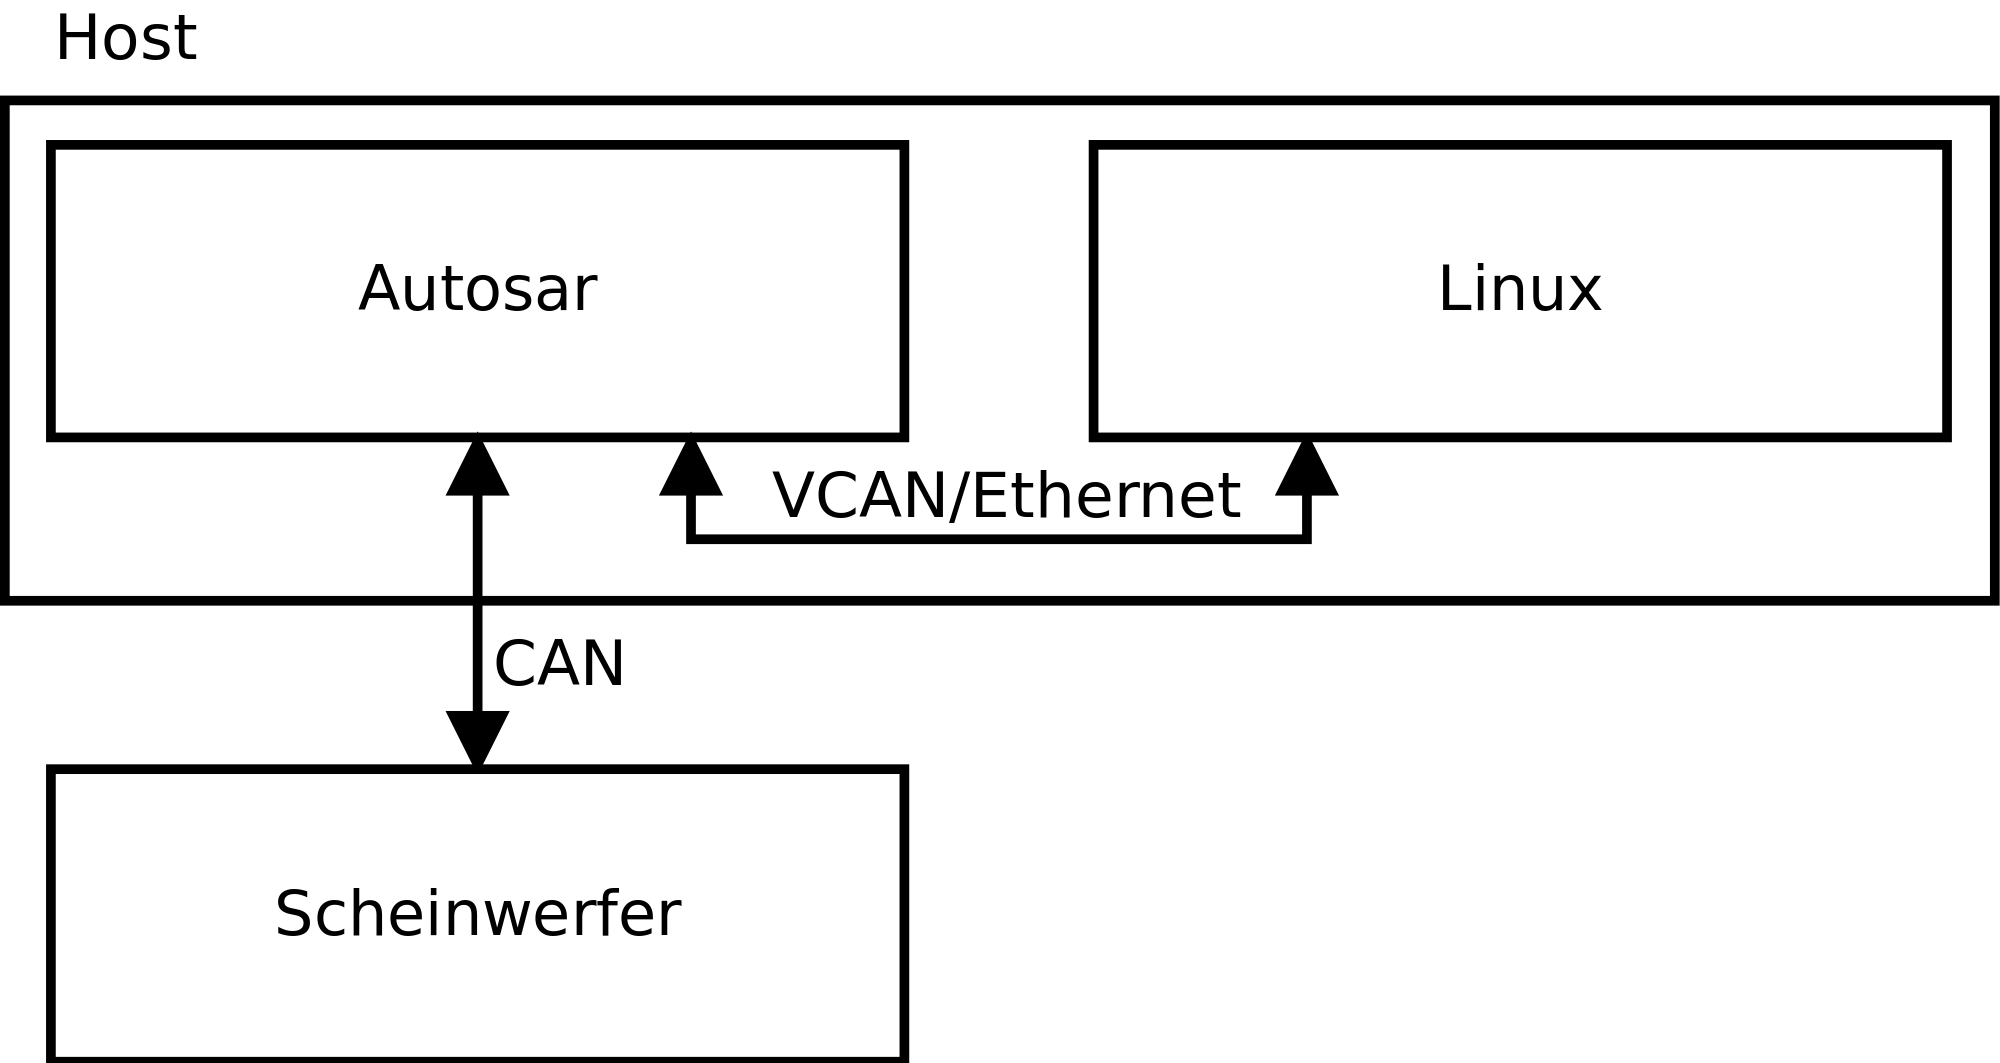
\includegraphics[width=0.8\textwidth]{overview.png}
\caption{Architektur}
\label{fig:arch}
\end{figure}

Die geplante Architektur der Scheinwerfer-Steuerung ist in Abbildung \ref{fig:arch} zu sehen. Dabei sind zwei getrennte Hardware Elemente zu sehen. Zum einen das Scheinwerfer-Steuergerät und zum anderen das in dieser Arbeit betrachtete System. Das Steuergerät übernimmt die direkte Steuerung der Scheinwerfer und ist per CAN-Bus mit dem anderen System verbunden.  Dieses beherbergt ein virtuelles AUTOSAR und Linux auf einem Windows Host.

Aus dieser Architektur-Beschreibung lassen sich vier Kern-Bereiche dieser Master-Arbeit ableiten:

\begin{itemize}
    \item Virtualisierung von AUTOSAR und Linux
    \item Kommunikation zwischen Linux und AUTOSAR
    \item Kommunikation zwischen AUTOSAR und Scheinwerfer
    \item Zugriff auf Hardware inklusive Betrachtung von Netzwerkmanagement
\end{itemize}

Hierbei ist zu beachten, dass das aktivieren des Netzwerkmanagements erst möglich ist, sobald eine Kommunikation zwischen AUTOSAR und der Hardware möglich ist.

% TODO: Projektplanung
Da der Zeitaufwand für die einzelnen Phasen nur sehr schwer einzuschätzen ist, wird für jede Phase des Projektes ein Monat Arbeit vorgesehen. Dazu kommen noch ein Monat Evaluation und Sicherheitsbetrachtung des Systems und zum Schluss ein Monat Fertigstellen der schriftlichen Arbeit. Die Zeitplanung ist in einem Gantt-Diagramm in Abbildung \ref{fig:gantt} zu sehen. Jede Phase enthält die Vorbereitung, Umsetzung und Dokmentation des entsprechenden Bereichs.


\begin{figure}[ht]
\centering

\begin{ganttchart}{12}
\gantttitle{2012}{8} 
\gantttitle{2013}{4} \\
\gantttitlelist{9,10,11,12,1,2}{2} \\
\ganttbar{Virtualisierung}{1}{2} \\
\ganttbar{Kommunikation Linux/AUTOSAR}{3}{4} \\
\ganttbar{Kommunikation AUTOSAR/Scheinwerfer}{5}{6} \\
\ganttbar{Zugriff auf Hardware}{7}{8} \\
\ganttbar{Evaluation}{9}{10} \\
\ganttbar{Fertigstellen der Arbeit}{11}{12} 
\end{ganttchart}

\caption{Zeitplanung Master-Arbeit}
\label{fig:gantt}
\end{figure}




%%%%%%%%%%%%%%%%%%%%%%%%%%%%%%% Grundlagen %%%%%%%%%%%%%%%%%%%%%%%%%%%%%%%%%%
\chapter{Grundlagen}
\label{sec:Grundlagen}
Dieses Kapitel enthält Grundlagen zu den Themen AUTOSAR und Virtualisierung. Dabei wird AUTOSAR ausführlich betrachtet, da es sich dabei um ein extrem umfangreiches Thema handelt. Zusätzlich ist dieser Teil der Arbeit als Einführung für zukünftige Arbeit im Bereich von AUTOSAR zu sehen.


%%%%%%%%%%%%%%%%%%%%%%%%%%%%%%% Virtualisierung %%%%%%%%%%%%%%%%%%%%%%%%%%%%%%%%%%
% Allgemeine Virtualisierung
% Class 1 und 2
\section{Virtualisierung}
\label{sec:Virtualisierung}
Der Begriff Virtualisierung bezeichnet eine Reihe von Techniken die verwendet werden um die Ressourcen eines Rechner-Systems zu verwalten. Hierdurch kann eine reales System als mehrere logische betrachtet und genutzt werden. Dabei können verschiedene Ziele verfolgt werden.

Aus dem Desktop-Bereich ist die System-Virtualisierung bekannt wie sie zum Beispiel mittels VirtualBox\footnote{VirtualBox zu finden unter \url{www.virtualbox.org}} umgesetzt ist. Hierbei werden die Ressourcen des bestehenden Systems durch einen Hypervisor verwaltet und den virtuellen Instanzen zugeordnet. Diese Art wird vor allem verwendet um zum Beispiel unter Windows Zugriff auf ein Linux zu haben um spezielle Software auszuführen.

Im Gegensatz dazu wird im Server-Bereich der Fokus auf andere Bereiche gelegt. Die hier verfolgten Ziele sind vor allem eine einfache Wartbarkeit, Ausfallsicherheit und Ressourcenschonung. Mittels virtueller Server können Ausfallzeiten minimiert werden, indem bei einem Ausfall einfach eine andere virtuelle Instanz des Servers gestartet wird und dessen Arbeit übernimmt. 

Virtualisierung kann mittels einer Reihe von Techniken erfolgen. Hier wird zum Beispiel Unterschieden ob die Hardware direkt zum Gast-System weitergegeben wird, oder aber eine eigene virtuelle Hardware emuliert wird. Außerdem könnte ein Gast-System Teile des Hosts, zum Beispiel dessen Kernel, mit verwenden. Allgemein werden die Hypervisor jedoch nach folgenden zwei Klassen unterschieden\cite[Seite 22 ff.]{hypervisor}:

\paragraph{Type 1 (bare host)} Hierbei handelt es sich um native Hypervisor die direkt auf der Hardware laufen. Diese bauen auf kein Betriebssystem auf und verwalten selbstständig die Ressourcen und Gast-Systeme. Aus diesem Grund sind sie vor allem Interessant für eingebettete Systeme. Type 1 Hypervisor werden genauer im nächsten Kapitel betrachtet.

\paragraph{Type 2 (extended host)} Ein Type 2 Hypervisor ist nur auf einem vollständigen Betriebssystem lauffähig. Damit ist der Hypervisor eine logische Schicht zwischen dem Host- und Gast-Betriebssystem und kann von den Vorteilen eines Betriebssystems profitieren. Hieraus ergibt sich das ein Type 2 Hypervisor meißt kleiner und schneller ist.





%%%%%%%%%%%%%%%%%%%%%%%%%%%%%%% Embedded Virtualisierung %%%%%%%%%%%%%%%%%%%%%%%%%%%%%%%%%%
% Gründe für Embedded Virtualisierung
\section{Virtualisierung bei eingebetteten Systemen}
\label{sec:EVirtualisierung}
Virtualisierung im Bereich der eingebetteten Systeme hat in den letzten Jahren immer mehr an Bedeutung gewonnen. Da Mikrocontroller und SOCs\footnote{System-on-a-Chip, dt. Ein-Chip-System} immer Leistungsfähiger werden ist es sinnvoll diese Leistung auch auszunutzen. Gerade im Automobil-Bereich, in dem die Anzahl der Steuergeräte zum Teil auf mittlerweile über 50 gestiegen ist, kann es die Kosten erheblich reduzieren wenn stattdessen einige dieser System virtualisiert werden können.

Hypervisor im embedded Bereich müssen bestimmte Erforderungen erfüllen die viele Hypervisor nicht betrachten. Zu diesen Anforderungen gehört zum Beispiel ein geringer Engerie-Verbrauch und Effiziente Speicher Nutzung. Ein weiterer wichtiger Punkt ist die Echtzeitfähigkeit. Diese ist vor allem kritisch, da meißt eine zwei-stufige Scheduler-Architektur entsteht, einmal der Scheduler des Hypervisors und einmal der Scheduler des Gast-Systems. Eine Echtzeit-Analyse ist in diesem Fall relativ anspruchsvoll.

Um nur ein einfaches Beispiel zu nennen, könnte ein System mit 4 Sub-Systemen betrachtet werden. Diese Sub-Systeme könnten alle in ein einziges System mit einer 4-Kern CPU vereint werden und genauso wie vorher verwendet werden. Je nach benötigter Leistung könnte das Resultierende System durchaus noch verkleinert und damit kostengünstiger gestaltet werden.


\subsection{Hypervisor Beispiel}
% Beispiele genauer betrachten: PikeOS, COQOS
% http://www.opensynergy.com/Products/COQOS
% http://www.windriver.com/products/hypervisor/
% http://www.ok-labs.com/products/okl4-microvisor
% http://www.lynuxworks.com/embedded-linux/embedded-linux-virtualization.php
% http://www.sysgo.com/products/pikeos-rtos-and-virtualization-concept/embedded-virtualization/
Im Bereich der Embedded Hypervisor gibt es eine Reihe verbreiteter Produkte. Dazu gehören zum Beispiel PikeOS\footnote{\url{http://www.sysgo.com/products/pikeos-rtos-and-virtualization-concept/embedded-virtualization/}}, OKL4\footnote{\url{http://www.ok-labs.com/products/okl4-microvisor}}, Integrity Multivisor\footnote{\url{http://www.ghs.com/products/rtos/integrity_virtualization.html}} und COQOS\footnote{\url{http://www.opensynergy.com/Products/COQOS}}.

% TODO: etwas zu den Beispielen schreiben



\subsection{Vorteile}
Der Einsatz von Virtualisierung bietet eine Reihe von Vorteilen\cite{wiki:emb_hyp}. Im folgenden werden davon einige näher betrachtet.

\paragraph{Betriebssystem Unabhängigkeit}
Da ein Hypervisor die Systeme vollständig trennt, ist es möglich verschiedene Betriebssysteme komplett parallel zu verwenden und die stärken der verschiedenen Systeme zu nutzen. So wird dieser Vorteil zum Beispiel bei COQOS genutzt um AUTOSAR und Android parallel lauffähig zu haben. Dadurch kann AUTOSAR Zeit- und Sicherheitskritische Aufgaben übernehmen und gleichzeitig Android den Infotainment Bereich verwalten.

\paragraph{Sicherheit}
Eine strickte Trennung durch Virtualiserung kann eine erhöhte Sicherheit bedeuten. Hierbei ist sowohl die Sicherheit vor Angriffen als auch Ausfällen gemeint. Zum einen ist eine Redundanz der Applikationen möglich. Diese Technik wird zum Teil in hochsicherheits Anwendungen, wie zum Beispiel Flugzeugen, genutzt um Code-Fehler auszuschließen. Es könnten also mehrere Applikationen mit unterschiedlichen Implementationen in verschiedenen VMs laufen.

Eine weitere Möglichkeit durch Virtualisierung die Sicherheit zu erhöhen ist das einsetzen eines Watchdog-Systems auf Hypervisor-Ebene. Dieser kann das korrekte Verhalten der VMs überprüfen und bei Bedarf ein System neu starten. Auch kann auf dieser Ebene eine Art Firewall implementiert werden. Diese könnte kontrollieren welche VMs welche Nachrichten senden und empfangen darf. Damit wird verhindert das zum Beispiel das Infotainment-System eine Motor-Relevante Botschaft auf den CAN-Bus schickt.

\paragraph{Wiederverwenden von altem Code}
Durch die Möglichkeit verschiedene Betriebssysteme einzusetzen, kann alter Code wiederverwendet werden. Damit kann die Zeit der Entwicklung reduziert werden und erst später das System auf ein neues Betriebssystem portiert werden.

\paragraph{IP Schutz und Trennung von Software Lizenzen}
Der Schutz von Intellectual Property spielt in der heutigen Wirtschaft eine große Rolle, jedoch bietet die Open-Source Welt einige Interessante Möglichkeiten. Um diese beiden Welten zu trennen und trotzdem von beidem zu profitieren, können unterschiedliche VMs verwendet werden. So ist es denkbar eine VM für jeglichen GPL-Code zu verwenden und die Kommunikation über Ethernet zu gestalten. Damit muss der eigene Code nicht auch unter der GPL freigegeben werden da nicht gegen GPL-Code gelinkt wurde.

\paragraph{Hypervisor klein und robust}
Ein im Embedded Bereich eingesetzter Hypervisor kann klein und robust sein, da die meißten der aus der Destop-Virtualisierung bekannten Techniken nicht benötigt werden. Daraus folgt das ein Embedded Hypervisor sehr kompakt sein kann und damit gut optimiert werden kann. Theoretisch ist es sogar möglich diesen Formal zu beweisen und somit auf dieser Ebene Sicherheit zu garantieren.

\subsection{Nachteile}
Natürlich bringt eine so umfangreiche Technik auch einige Nachteile mit, von denen einige im folgenden betrachtet werden.

\paragraph{Single Point of Failure}
Da der Hypervisor eine zentrale Position besitzt, kann ein Ausfall dessen das gesamte System gefährden. Da der Hypervisor für die Ausführung der Instanzen verantwortlich ist, und auch den Speicher und Kommunikations-Dienste verwaltet, würde ein Fehler oder sogar ein Ausfall des Hypervisors, ein Ausfall des Gesamt-Systems verursachen. Dementsprechend ist der Hypervisor nach den höchsten Ansprüchen der Sicherheits-Technik zu entwerfen. Zudem sollten umfangreiche Diagnose-Möglichkeiten vorhanden sein, um das Risiko eines unerwarteten Ausfalls zu minimieren.

\paragraph{Performance Overhead}
Durch das Einsetzen eines Hypervisors und mehreren VMs kann es zu einem Performance Overhead kommen. Dieser kann jedoch minimiert werden indem die Hardware entsprechend gewählt wird. So bieten moderne CPU-Architekturen verschiedene Virtualisierungs-Eweiterungen mit denen der Overhead minimiert wird. Auch eine angemessene Anzahl der CPU-Kerne kann den Overhead minimieren indem Preemption zwischen den VMs verhindert wird.

\paragraph{Weniger Hardware-Redundanz}
Da sich die Anzahl der Steuergeräte durch Virtualisierung verringert, verringert sich auch die Hardware-Redundanz. In dem Extrem-Beispiel indem nur noch ein Steuergerät im Auto vorhanden wäre, würde ein Single-Point-of-Failure existieren und so die Sicherheit stark gefährden. Auf der anderen Seite könnte dieser Nachteil jedoch durch Virtualisierung auch stark verbessert werden. So ist es möglich das ein anderes Steuergerät einen Ausfall erkennt und direkt eine Ersatz-VM startet um so die Sicherheit weiter zu gewährleisten. 





% TODO
%%%%%%%%%%%%%%%%%%%%%%%%%%%%%%% Allgemeine Softwarearchitektur %%%%%%%%%%%%%%%%%%%%%%%%%%%%%%%%%%
%\section{Allgemeine Softwarearchitektur}
%\label{sec:allg_softarch}
% System, Komplexität, Partitionierung

% Um Nutzen von Autosar verstehen zu können: System verstehen
% Beispiel System 'Auto': Mechanik, Hardware und Software; Autosar übernimmt Software
% Allgemeine Begriffe: System, Struktur, Komplexität, 
% Beispiel für Systeme
% System partitinieren
% Begriff Architektur
% Anfoerdungens
% Abstraktion
% Schichten architektur
% Komponenten Architektur







%%%%%%%%%%%%%%%%%%%%%%%%%%%%%%% Autosar %%%%%%%%%%%%%%%%%%%%%%%%%%%%%%%%%%
\section{AUTOSAR}
\label{sec:Autosar}
Bei AUTOSAR handelt es sich um eine offene und standardisierte Softwarearchitektur die Hauptsächlich in der Automobil-Industrie Verwendung findet. AUTOSAR, kurz für \emph{AUTomotive Open System ARchitecture}, wurde gemeinsam von einer Reihe von Automobilherstellern und Zulieferern seit etwa 2003 entwickelt. Zu den Kern Mitgliedern gehören zur Zeit BMW, Bosch, Toyota, Volkswagen und eine Reihe anderer. AUTOSAR ist als Erbe von OSEK/VDX zu sehen und baut somit auch zum Teil auf dieses auf.

Gemäß dem AUTOSAR-Leitspruch "`Cooperate on standards, compete on implementation"' handelt es sich bei AUTOSAR lediglich um einen Standard. Ziel von AUTOSAR ist es Schnittstellen zu definieren die möglichst alle Vorrausetzungen der Automobilindustrie erfüllen und damit den Standard allgemein Einsetzbar machen. Die Implementation des AUTOSAR-Standards ist den verschiedenen Firmen überlassen. Im Kapitel \ref{sec:Toolkette} wird eine kurze Übersicht der verschiedenen AUTOSAR-Distributionen und zugehöriger Tools gegeben.

Im folgenden Kapitel wird ein kurzer Überblick der Technik von AUTOSAR gegeben. Um den Rahmen dieser Arbeit nicht zu sprengen beschränkt sich das Kapitel auf die Grundlagen und wichtigsten Konzepte. Ein übersichtlicher und guter Einblick ist in \cite{autosar_techoverview} und \cite{autosar_layer} zu finden.

Ein Grund für den Einsatz von AUTOSAR ist vor allem die steigende Komplexität von Elektrik/Elektronik Systemen (kurz E/E Systeme) wie sie im Automobil Umfeld vorkommen. Um diese Komplexität auch in Zukunft noch verwalten zu können bedarf es eines Standard-Systems das genau auf diese Bedürfnisse zugeschnitten ist. Weitere Ziele die AUTOSAR verfolgt sind Flexibilität, Skalierbarkeit, Qualität und Zuverlässigkeit. \cite[S. 5]{autosar_techoverview}

\begin{table}[h]
\center
\begin{tabular}[h]{c c c l}
\toprule
Release & Datum & Phase & Notiz\\
\midrule
      & Juli 2003  &  & Gründung AUTOSAR\\
\midrule
1.0   & 08.07.2005 & \multirow{3}{*}{Phase I} & \\
2.0	  & 04.05.2006 &  & Entwicklung des Standards\\
2.1	  & 04.12.2006 &  & \\
\midrule
3.0	  & 21.12.2007 & \multirow{3}{*}{Phase II} & \\
3.1	  & 15.08.2008 &  & Selektive Verbesserungen\\
4.0	  & 18.12.2009 &  & \\
\midrule
4.0.2 & 15.04.2011 & \multirow{3}{*}{Phase III} & \\
3.2	  & 13.05.2011 &  & Wartung\\
4.0.3 & 22.12.2011 &  & \\
\bottomrule
\end{tabular}
\caption{Zeitlicher Ablauf der AUTOSAR-Entwicklung (vgl. \cite{wiki:autosar_de}\cite{as_roadmap}\cite{as_background})}
\label{tab:timeline}
\end{table}

% TODO: Text zur Zeitleiste
Tabelle \ref{tab:timeline} zeigt die Versions-Historie von AUTOSAR. 






\subsection{Grundkonzepte}
\label{sec:Grundkonzepte}
Diese Kapitel soll einen Überblick über die Grundlagen von AUTOSAR geben. Anhand der Abbildung \ref{fig:autosar_overview} werden im folgenden die verschiedenen Aspekte von AUTOSAR betrachtet. Dieses Kapitel basiert stark auf \cite{autosar_techoverview}.

\begin{figure}[!htbp]
    \centering
    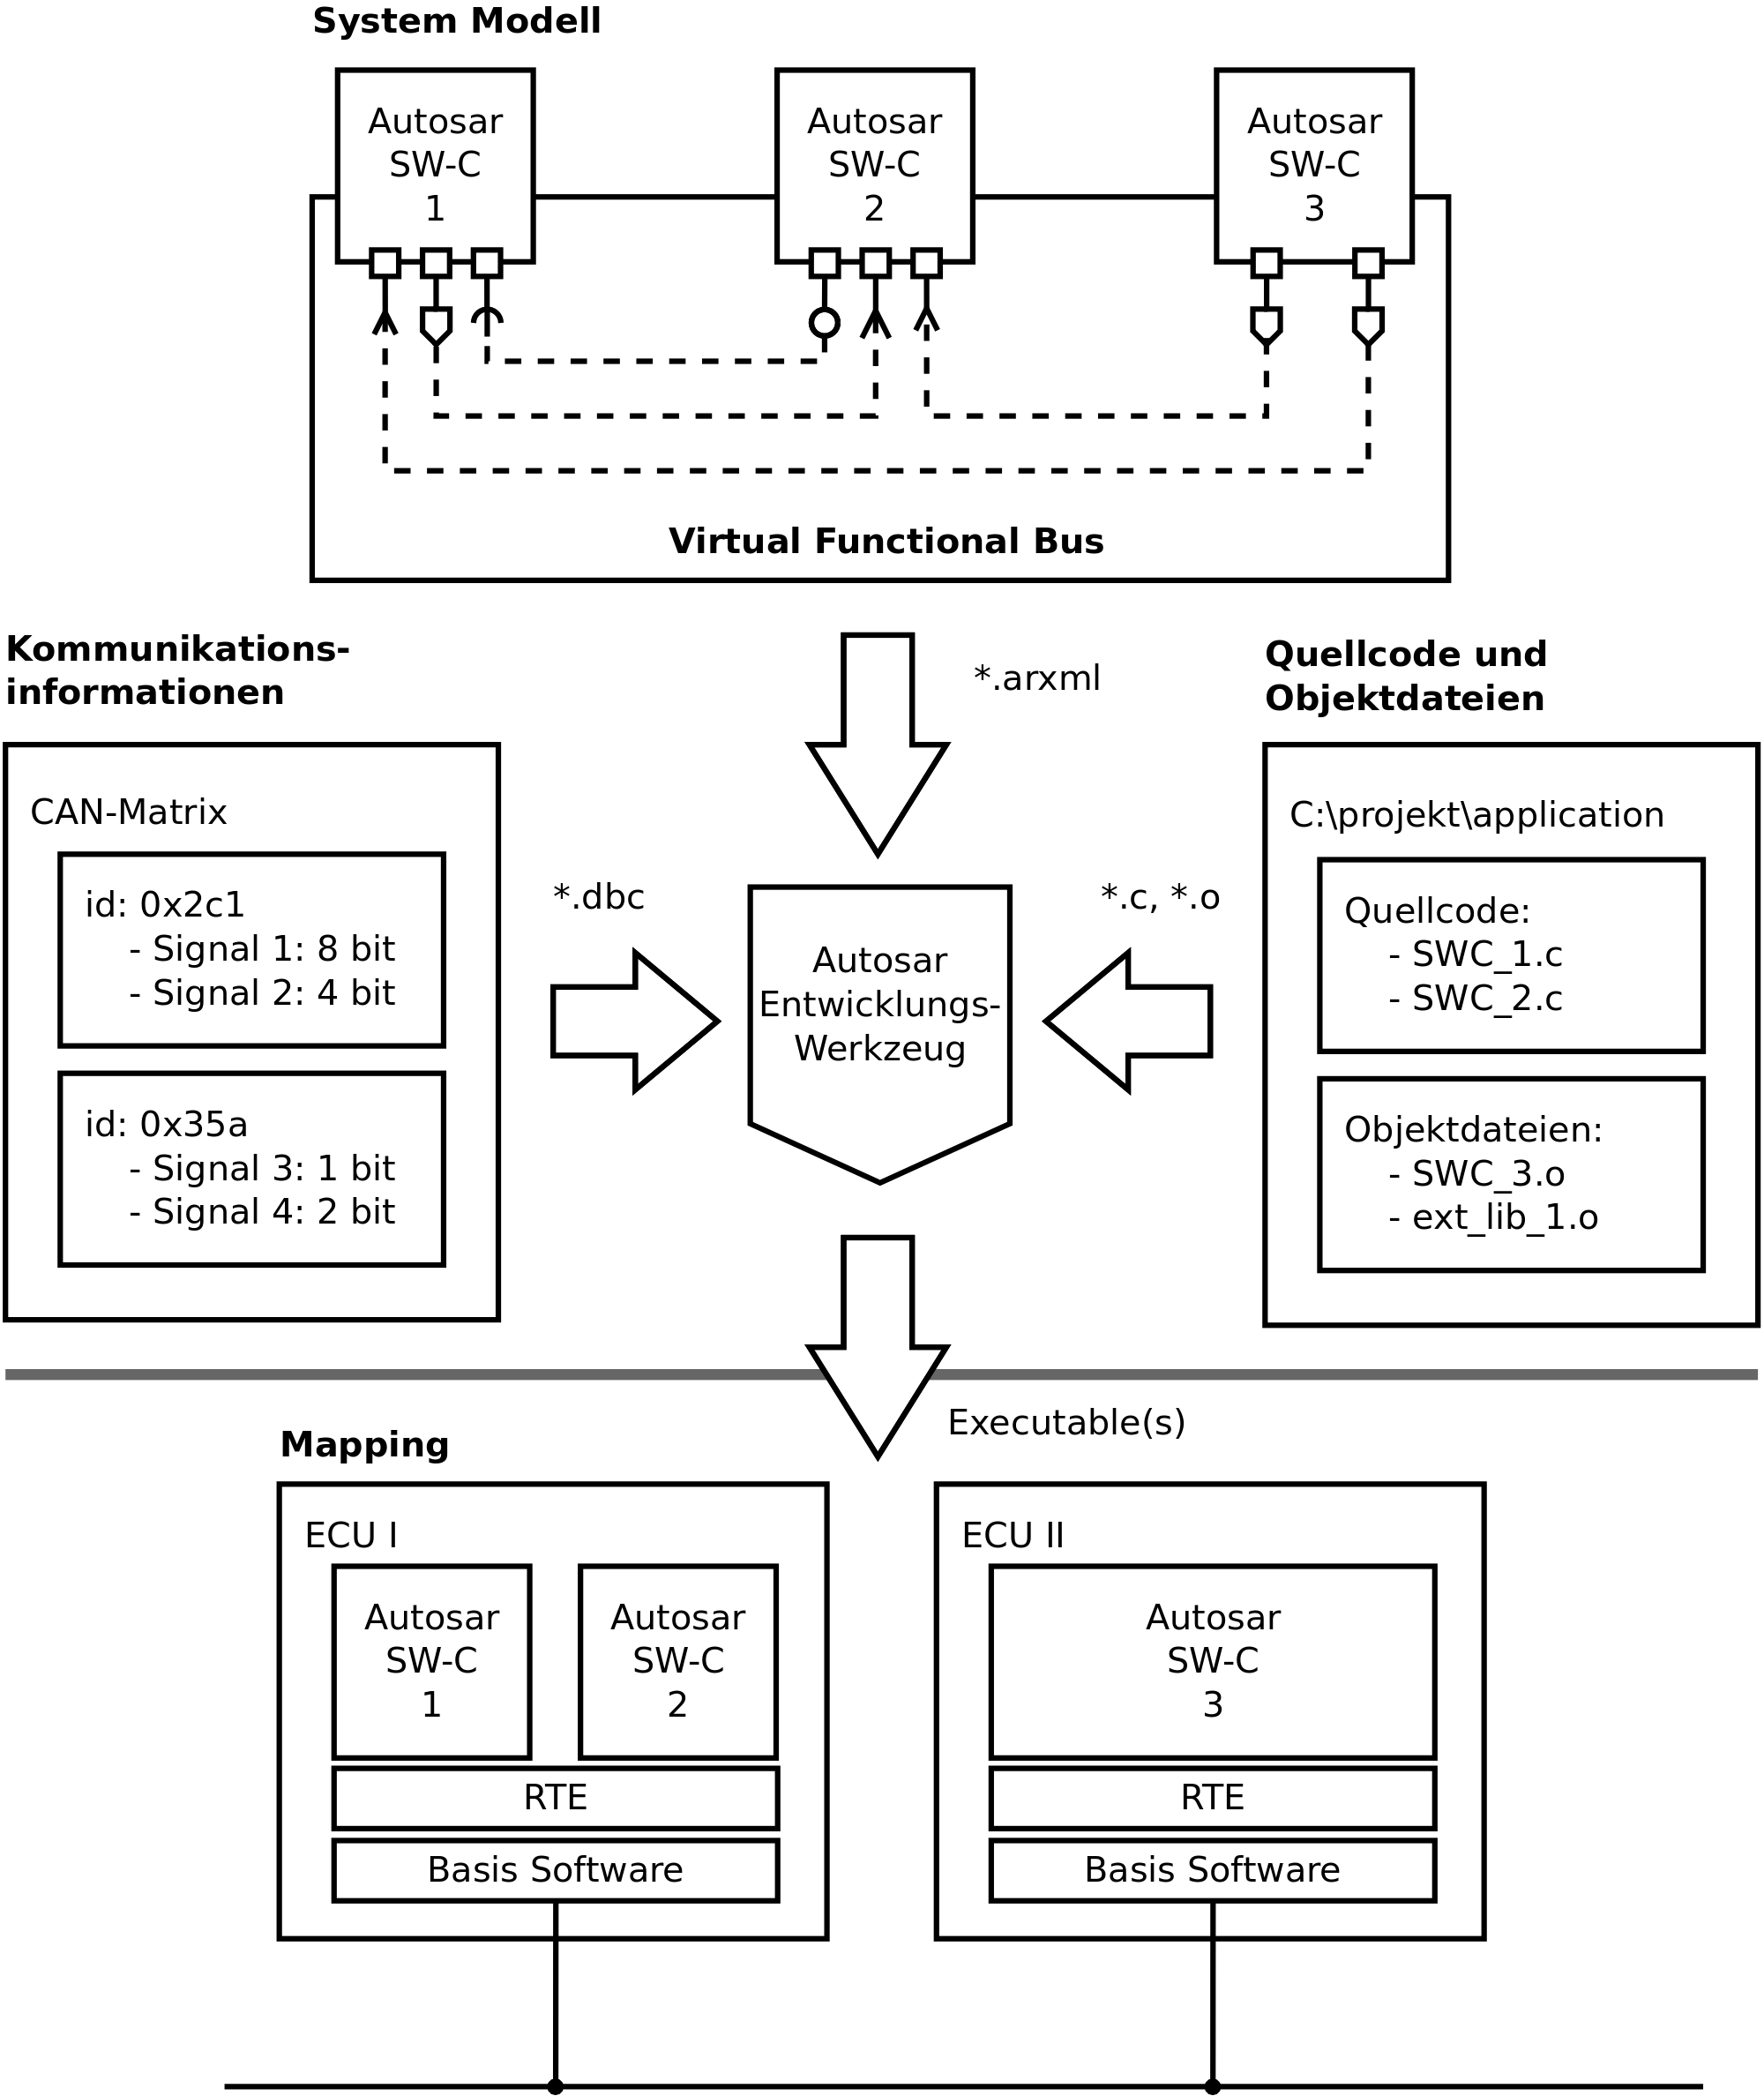
\includegraphics[width=1\textwidth]{autosar_overview.png}
    \caption{Autosar Überblick}
    \label{fig:autosar_overview}
\end{figure}

Der Lebenszyklus eines AUTOSAR Systems lässt sich in zwei Phasen unterteilen. Die erste Phase ist in der Abbildung im oberen Teil zu sehen und beinhaltet das Design und die Entwicklung. In der zweite Phase werden alle Konfigurationen und Quelldateien verwendet um mittels des "`AUTOSAR Entwicklungswerkzeugs"'  ausführbare Dateien zu generieren, die anschließend auf der Ziel-Hardware ausgeführt werden können. Im folgenden werden die einzelnen nötigen Elemente näher erläutert.


\paragraph{System Description} Ein Entwurf der "`System Description"' ist am oberen Rand der Abbildung zu sehen. Hier werden Komponenten und deren Verbindungen definiert. Die verschiedenen Interfaces und der Virtual Functional Bus werden in einem seperaten Abschnitt näher betrachtet. Komponenten (Software-Components, kurz SW-C) können beliebig geschachtelt werden um so eine logische Trennung zwischen Teil-Systemen zu schaffen. Hierbei ist lediglich zu beachten, dass pro ECU eine Top-Level-Composition (kurz TLC) gefordert wird. Die eigentliche Funtkionalität ist in Runnables implementiert. Diese müssen einer SW-C zugehören und werden von einem RTE-Event, zum Beispiel ein Timer, aktiviert.

Der Entwurf des Systems sollte genau überlegt sein, da dieser Grundstein für die weitere Entwicklung ist. In dieser Phase erfolgt auch die Zuriffskontrolle auf Interfaces sowie die Definition der RTE-Events, Zugriff auf Inter-Runnable-Variables und einer Reihe weitere Eigenschaften die später relevant sind.

Als Austauschformat wird XML, mit der Dateiendung "`.arxml"' verwendet. Es ist möglich nur einen Teil des Systems in eine XML-Datei zu exportieren um zum Beispiel einem OEM nur die für ihn relevante Teile offenzulegen.

Innerhalb dieses Projektes wird Systemdesk der Firma dSpace verwendet.

\paragraph{Kommunikations-Informationen}
Um eine Kommunikation zwischen mehreren Komponenten zu ermöglichen müssen entsprechende Informationen geliefert werden. Hierbei existieren zum Beispiel die Formate DBC, FIBEX und LDF. Obwohl es sich bei DBC und LDF prinzipiell um Bus-Systemabhängige Formate handelt, spielt dies bei AUTOSAR keine Rolle. So wird im AUTOSAR-Stack die Kommunikations derart abstrahiert, sodass Botschaften transparent über unterschiedliche Bus-Systeme oder auch innerhalb einer ECU übertragen werden können.

Relevante Informationen sind Botschaften-IDs, Bezeichner, Bitlänge und Position der Signale in der Botschaft. Im Rahmen dieses Projektes werden DBC-Dateien mittels Vector CANoe erstellt.

\paragraph{Quellcode und Objektdateien}
Die eigentliche Implementation der Funktionalität findet im Quellcode, beziehungsweise im Objektcode statt. Durch den AUTOSAR-Standard ist ein Benennungsschema definiert, wodurch die entsprechenden Funktionen identifiziert werden. Auch der Zugriff auf Funktionen der RTE sind durch dieses Schema definiert. Die API-Funktionen der RTE werden vom RTE-Generator der verwendeten AUTOSAR-Distribution erstellt.

\paragraph{AUTOSAR Entwicklungswerkzeug}
An zentraler Stelle in der Abbildung steht das "`AUTOSAR Entwicklungswerkzeug"'. Dies besteht genau genommen aus mindestens drei Teilen und muss nicht zwingend komplett von einem Hersteller stammen. So gibt es einige Implementationen die nur einen Teil des Aufgabenbereichs abdecken. Die drei nötige Komponenten sind:

\begin{itemize}
    \item Basis-Software Implementation
    \item Basis-Software Konfigurator
    \item Runtime-Enviroment Generator
\end{itemize}

\begin{figure}[!htbp]
    \centering
    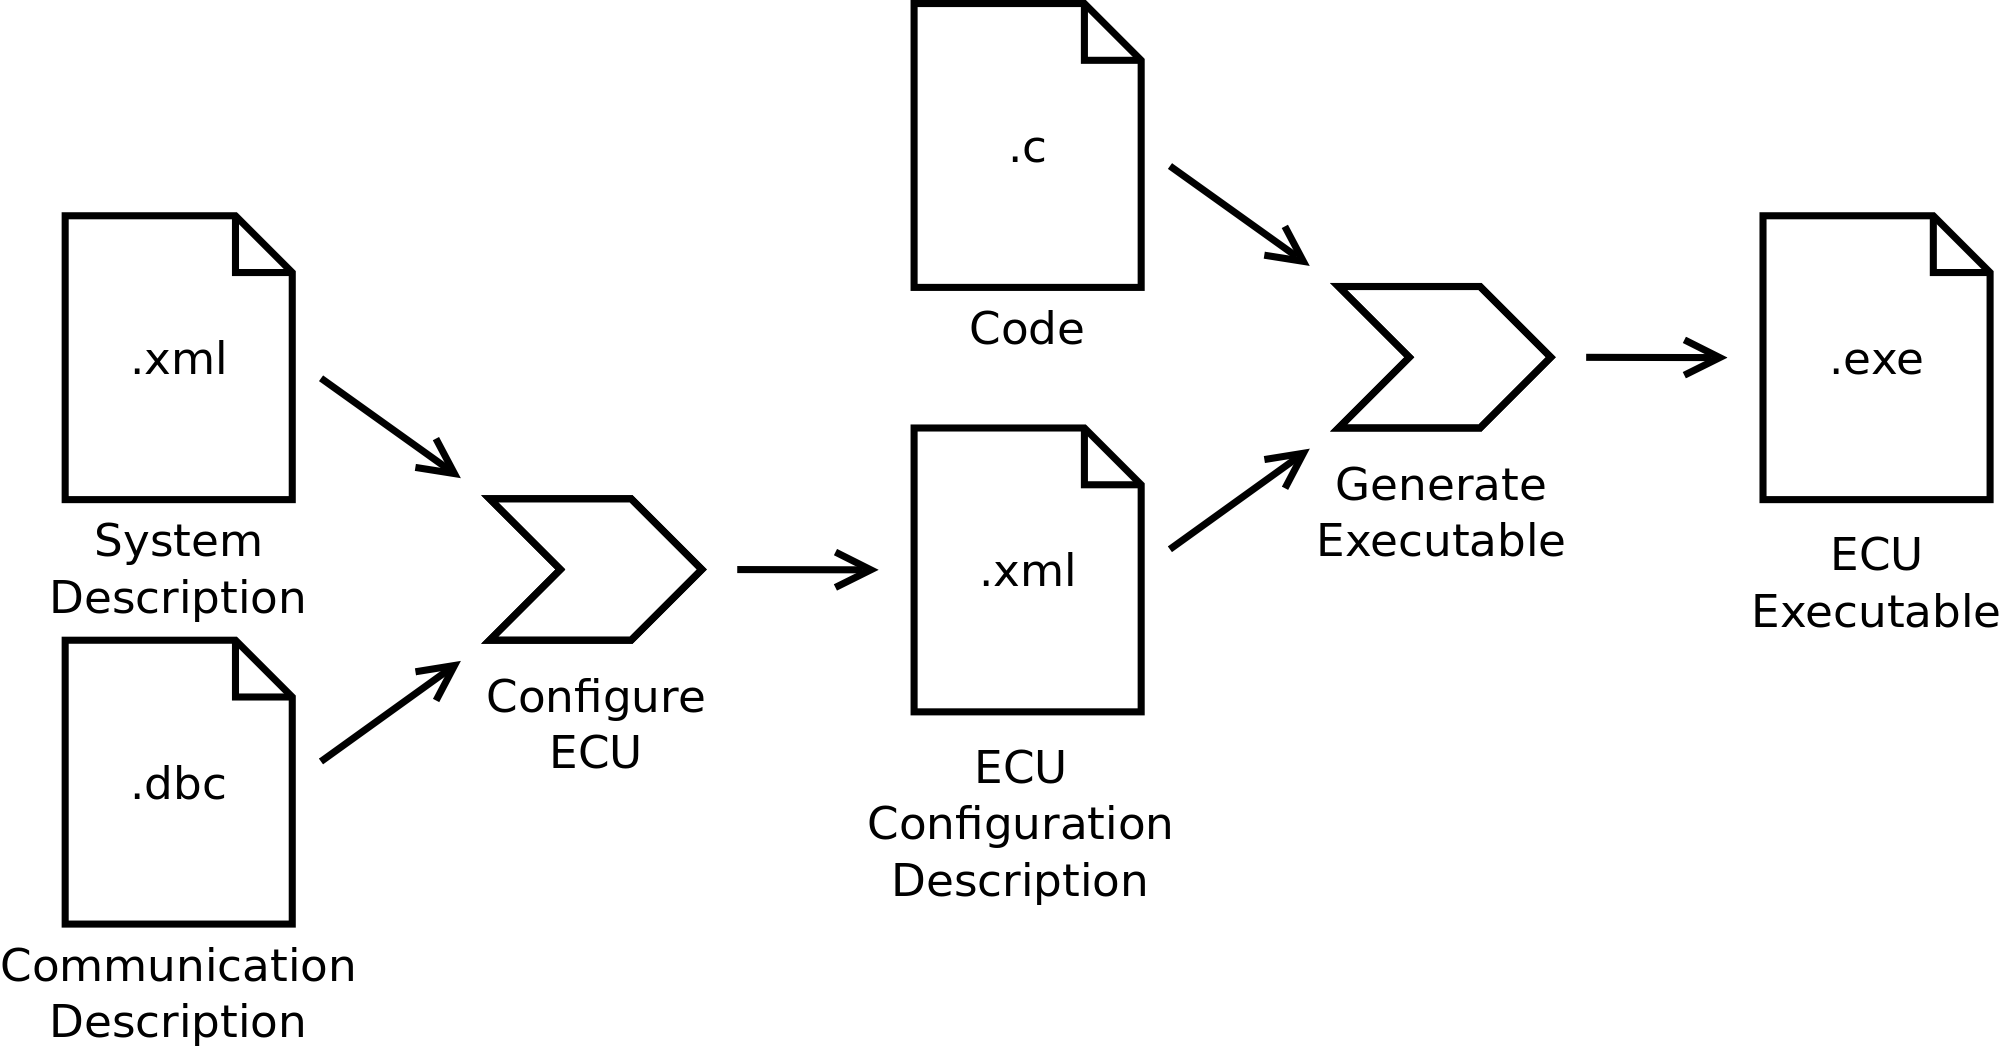
\includegraphics[width=1\textwidth]{Autosar_Prozess.png}
    \caption{AUTOSAR-Entwicklungs-Prozess}
    \label{fig:autosar_prozess}
\end{figure}

Die Basis-Software Implementation stellt das eigentliche Betriebssystem, inklusive aller Module dar. Mit Hilfe des Basis-Software Konfigurators werden die verschiedenen Module des Betriebssystems ausgewählt und konfiguriert. An dieser Stelle werden zum Beispiel Tasks erstellt und Botschaften-IDs vergeben. Zu diesem Zweck kann an dieser Stelle die System- und Kommunikations-Beschreibung importiert werden. Hierdurch können einige Einstellung automatisch vorgenommen werden. Der letzte Teil der AUTOSAR-Entwicklungsumgebung ist der RTE-Generator. Dieser benötigt eine System-Beschreibung und generiert aus dieser die entsprechende API zwischen BSW und Applikation. Der vereinfachte AUTOSAR-Entwicklungs-Prozess ist in Abbiludng \ref{fig:autosar_prozess} zu sehen.



\subsection{Virtual Functional Bus und Runtime-Enviroment}
\label{sec:vfb}
Eines der Kernkonzepte zur Kommunikation und zur Abschottung der User-Applikation ist der "`Virtual Functional Bus"' (kurz VFB) und die "`Runtime-Enviroment"' (kurz RTE). Durch diese soll ein Austausch und eine Verlagerung auf eine andere ECU ermöglicht werden. Dies wird ermöglicht durch eine vollständige Trennung zwischen der Basis-Software und der User-Applikation wie es in Abbildung \ref{fig:autosar_layer} zu sehen ist. 

\begin{figure}[!htbp]
    \centering
    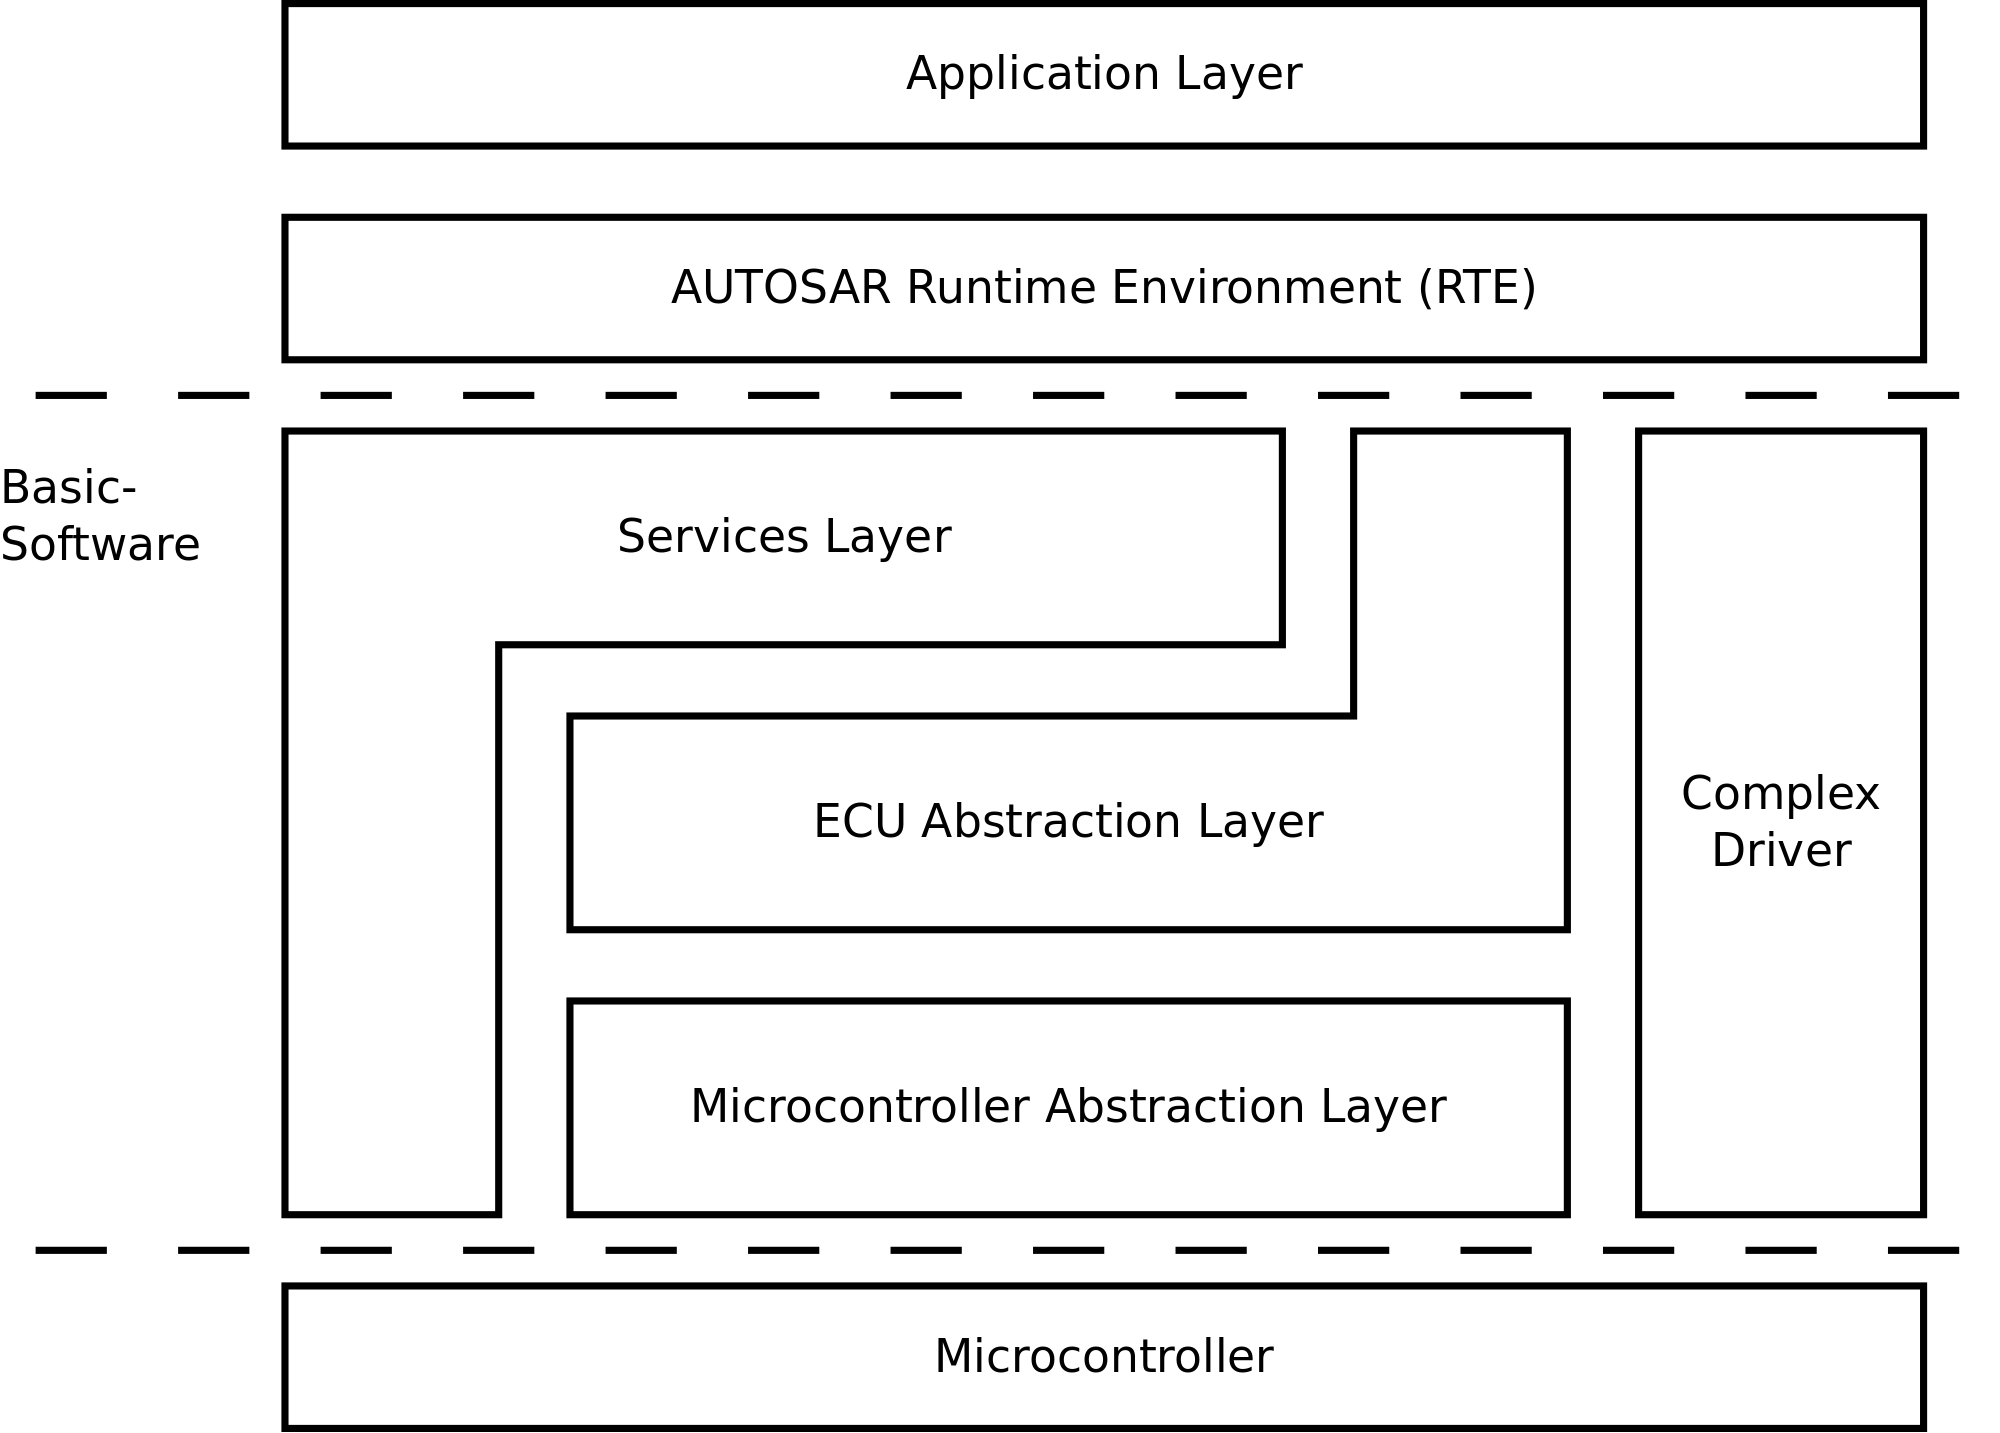
\includegraphics[width=1\textwidth]{autosar_layer.png}
    \caption{AUTOSAR Schichtenmodell}
    \label{fig:autosar_layer}
\end{figure}

Wie der Name schon sagt, handelt es sich beim VFB um einen virtuellen Bus. Aus diesem Grund ist dieser auch nicht in Abbildung \ref{fig:autosar_layer} zu sehen. Dies ergibt sich aus einer Trennung zwischen Design-Phase und Compilezeit bzw. Laufzeit. So wird während der System-Modellierung der VFB entworfen, der später zu einer oder mehreren RTEs wird. Mit Hilfe des VFB wird die Kommunikation zwischen den verschiedenen Komponenten ermöglicht. So werden Möglichkeiten geboten verschiedene Interface-Typen und Ports zu definieren. Bei Ports handelt es sich um Interaktionspunkte zwischen Softwarekomponenten. Dabei wird zwischen PPorts (provide ports), die etwas bereitstellen, und RPorts (require ports), die etwas benötigen, unterschieden. Um einen Port verwenden zu können muss diesem ein Port Interface zugeordnet sein.

Die zwei wichtigsten Interfaces werden im weiteren kurz betrachtet. Analog zu diesen existieren noch zwei AUTOSAR-Service-Interfaces, die AUTOSAR-intern verwendet werden. Also zum Beispiel ein Aufruf zum ECU-State-Manager (EcuM). Außerdem wird noch ein Kalibrierungs-Interface angeboten, mit Hilfe dessen sich statische Kalibrierungs-Daten bereitstellen und abfragen lassen. Zusätzlich kann beim Zugriff auf ein Port zwischen einem Expliziten und Impliziten Zugriff unterschieden werden. Diese Modi, sowie die Multiplizität der Interface soll an dieser Stelle nicht erläutert werden und ist unter \cite[Seite 101 ff.]{SE_Autosar} nachzulesen.

\paragraph{Sender/Receiver Interface}
Bei einem Sender/Receiver Interface handelt es sich um einen Kommunikationsmechanismus mit dessen Hilfe Daten ausgetauscht werden können. Die übertragenen Daten können dabei sowohl primitve als auch komplexe Datentypen wie Strukturen enthalten.

\paragraph{Client/Server Interface}
Vom Server wird hier eine Funktion bereitgestellt, die vom Client aufgerufen werden kann. Dabei können mit Hilfe der Übergabe- und Rückgabeparameter auch Daten ausgetauscht werden.

\paragraph*{}
Bei der RTE handelt es sich um eine konkrete Implementierung des VFB. Während der VFB zur Design-Phase das komplette Modell abdeckt, wird eine RTE pro ECU verwendet. Diese RTE stellt alle Methoden zur Verfügung, die für die Kommunikation der Komponenten dieser ECU nötig sind. Das bedeutet das auf alle Methoden verzichtet wird, die auf dieser ECU nicht ausgeführt werden können.

Die angebotenen Schnittstellen werden bei der Generierung der RTE erstellt, und folgen definierten Namensschemata. Im folgenden werden ein paar Beispiel kurz betrachtet. Die genaue Benennung der Schnittstellen ist in der Spezifikation nachzulesen.

\begin{lstlisting}[frame=single, basicstyle=\footnotesize, caption={RTE Beispiele}, label={lst:rte_beispiele}]
Std_ReturnType Rte_Write_<p>_<d>(IN Rte_Instance <self>, IN <data>)
Std_ReturnType Rte_Read_<p>_<d>(IN Rte_Instance <self>, OUT <data>)
\end{lstlisting}

Die in Zeile 1 und 2 in Listing \ref{lst:rte_beispiele} gezeigten Beispiele, werden verwendet, um auf ein Sender/Receiver-Interface zuzugreifen. Dabei stehen die Platzhalter \texttt{<p>} und \texttt{<d>} für den entsprechenden Port und das gewünschte Datenelement. Das Argument \texttt{<data>} entspricht dem zu empfangen beziehungsweise zu sendenden Datenelements. Das Element \texttt{<self>} vom Typ Rte\_Instance wird verwendet um mehrere Instanzen zu verwalten und funktioniert ähnlich wie ein \texttt{this}-Pointer bei der Objekt-Orientierung.

Das Hauptkonzept der Techniken VFB und RTE ist die Festlegung von Schnittstellen. Dieses Konzept wird bereits seit langer Zeit in anderen Bereichen der Software-Entwicklung durchgeführt. So werden zum Beispiel bei Java Interfaces verwendet, um konkrete Implementationen abzukapseln und generisch zu halten. 

Diese Konzepte werden beim VFB und der RTE eingesetzt um SW-Cs austauschbar zu halten. Somit soll es möglich sein, eine Implementation einer SW-C durch eine andere auszutauschen, ohne das Gesamt-System zu verändern. Zudem ist ein Ziel, die Funktionalität unabhängig von der Hardware zur Verfügung zu stellen. Das bedeutet das eine SW-C auf eine andere ECU verlagert werden kann, ohne weitere Anpassungen vornehmen zu müssen. Dabei müssen lediglich die RTE-Schichten neu generiert werden, um damit zum Beispiel Intra-ECU Kommunikation zur Inter-ECU Kommunikation zu verändern. Ob dieses Verfahren in der Praxis so einfach eingesetzt werden kann, ist zweifelhaft. So muss die für die SW-C nötig Hardware (zum Beispiel PWM-Ausgänge) sowohl vorhanden sein, als auch bei der ECU-Konfiguration korrekt eingerichtet sein. Zudem müssen entsprechende Timer konfiguriert sein, um die enthaltenen Runnables ausführen zu können. Allgemein gilt jedoch, dass durch die Kapselung ein Austausch der Software erleichtert wird.









\subsection{Basis-Software}
\label{sec:bsw}
Bei der Basis-Software (kurz BSW) handelt es sich um das eigentlich Betriebssystem. Dieses stellt verschiedene Funktionen bereit. Darunter zum Beispiel ein Scheduler und eine Verwaltung der Tasks. Außerdem sind eine Hardware-Abstraktion und -Treiber hier untergebracht. Dabei ist das gesamte System modular aufgebaut um möglichst Übersichtlich zu sein. Abbildung \ref{fig:autosar_refined_layer} zeigt die grobe Struktur der Basis-Software. Die genaue Einteilung der Module und Abhängigkeiten zwischen diesen wird im Rahmen dieser Arbeit nicht beschrieben. Der geneigte Leser findet jedoch unter \cite{autosar_layer} nähere Informationen dazu.

\begin{figure}[!htbp]
    \centering
    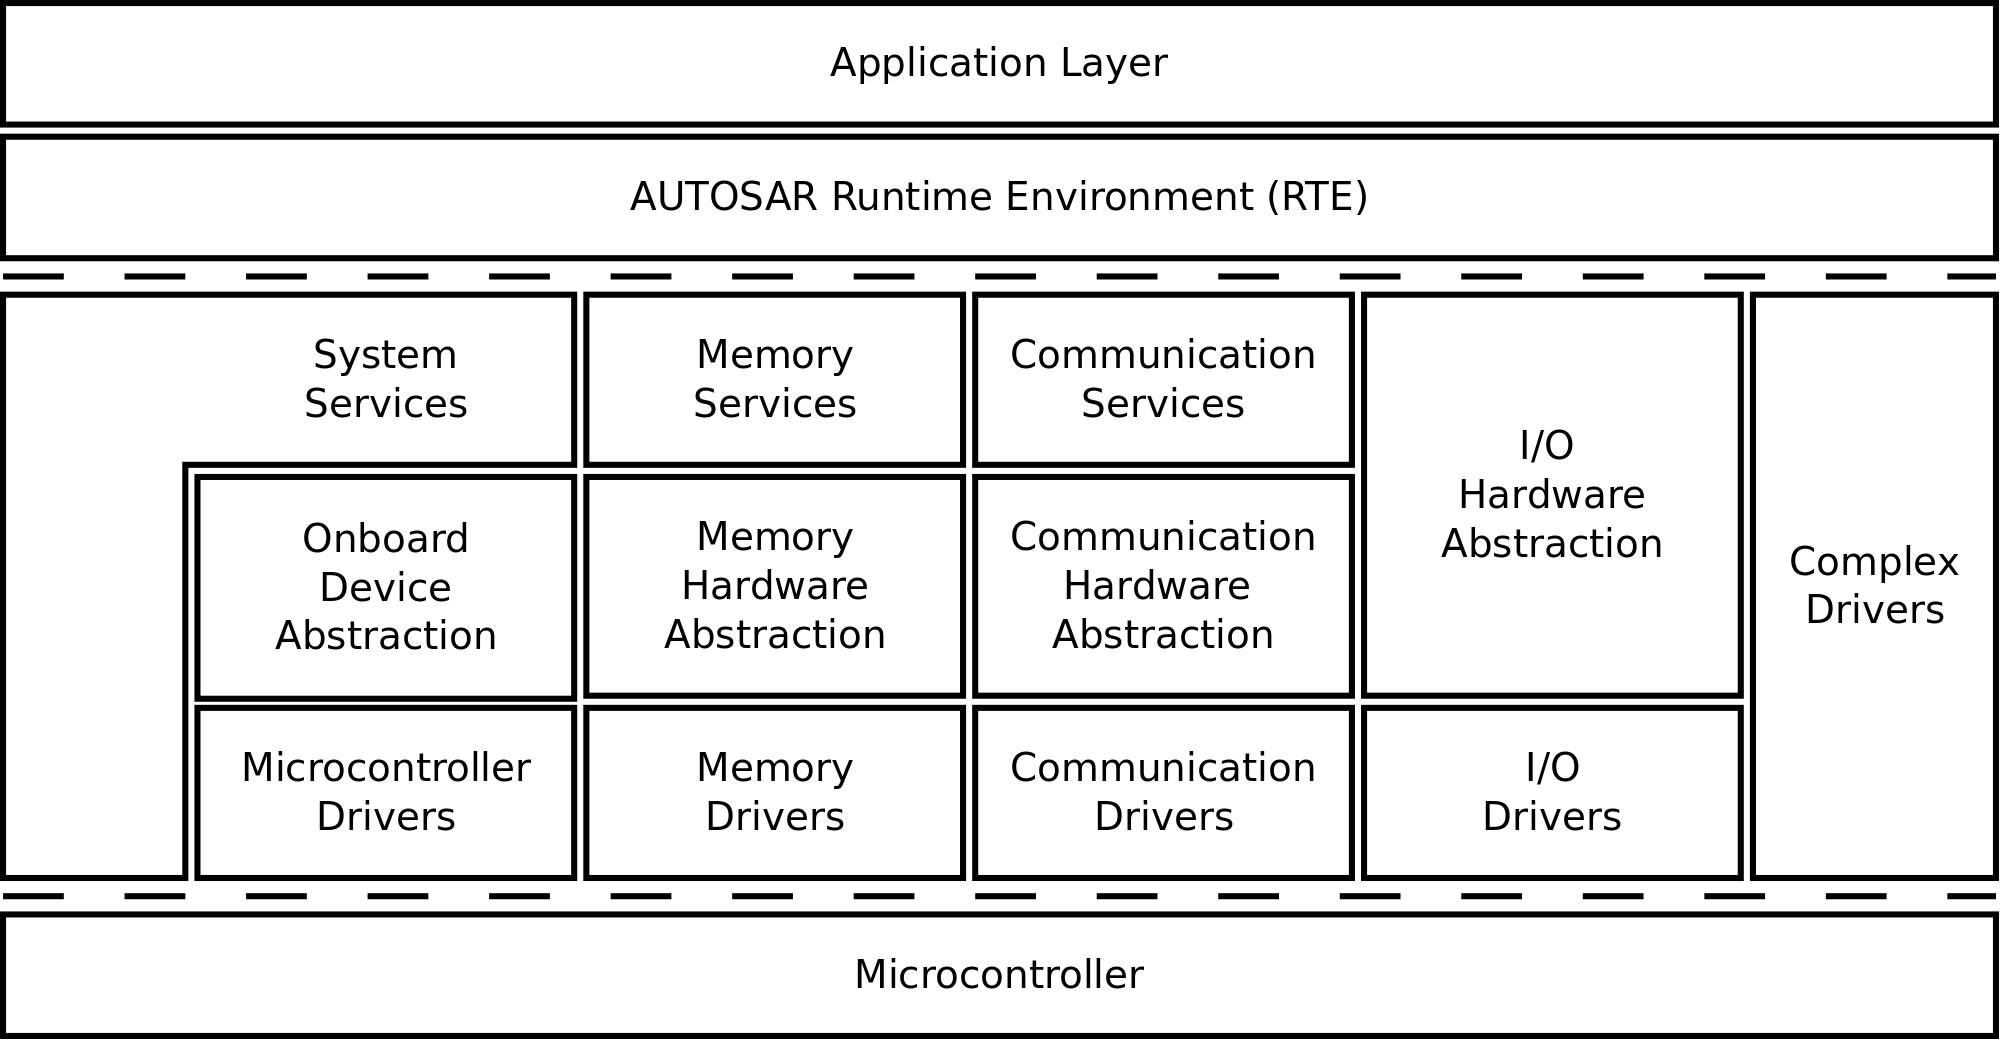
\includegraphics[width=1\textwidth]{autosar_refined_layer}
    \caption{AUTOSAR Schichtenmodell mit genauerer Aufteilung}
    \label{fig:autosar_refined_layer}
\end{figure}

AUTOSAR, und damit auch das Betriebssystem und die Basis-Software, ist als statisches System entworfen. Das bedeutet das alle Entscheidungen und Einstellung zur Entwicklungs-Zeit feststehen müssen. Somit können nach der Compile-Zeit keine Veränderungen am System vorgenommen werden. Auch ist dynamisches Linken von Komponenten oder dynamische Speicheranforderung nicht möglich. Hierdurch wird die Komplexität des Systems möglichst gering gehalten, und damit die Analyse, vor allem im Bezug auf Echtzeitfähigkeit, vereinfacht.\cite[Seite 186]{SE_Autosar}

Der modulare Aufbau der BSW bietet einige interessante Vorteile. So ist der Umfang eines Moduls, und damit alle Rechte und Pflichten, durch die Spezifikation klar vorgegeben. Dadurch sind Module austauschbar und einfach testbar. Zusätzlich besteht so die Möglichkeit, einzelne Module von verschiedenen Herstellern zu beziehen. Damit hat ein BSW-Anbieter die Möglichkeit sich auf bestimmte Module oder Modul-Gruppen zu beschränken oder zu spezialisieren. Auch ist es vorstellbar, dass ein Automobil-Hersteller eine konkrete Implementation einiger Module verlangt. So könnte gefordert werden, dass der gesamte Kommunikations-Stack immer von einem Hersteller stammt um absolute Kompatibilität zu gewährleisten.

Durch die starke Modularisierung entstehen jedoch auch ein erhöhter Kommunikationsaufwand. Vor allem in Zeitkritischen Applikationen kann dies ein Nachteil darstellen. Die von AUTOSAR vorgesehene Lösung für dieses Problem sind die \emph{Implementation Conformance Classes}, kurz ICC. Diese mit ICC 1, ICC 2 und ICC 3 benannten Klassen geben Auskunft über die Granulität der Basissoftware. ICC 3 stellt dabei eine Basis-Software dar, bei der alle Module entsprechend der Spezifikation gegliedert und implementiert sind. Bei der Klasse ICC 2, können mehrere Module zu einem Cluster zusammengefasst werden. Dabei müssen nur die Schnittstellen zu den außerhalb liegenden Modulen beziehungsweise Modul-Clustern der Spezifikation entsprechen. Als letzte Klasse stellt die ICC 1 ein einziges Cluster dar. Hier kann die gesamte Basis-Software als proprietärer Gesamtblock gesehen werden. Dabei müssen nur die Schnittstellen zur RTE entsprechend dem Standard definiert sein. Dies kann als Möglichkeit zur Migration von bestehenden Systemen genutzt werden, indem zu erst nur die RTE AUTOSAR-konform eingeführt wird. Zusätzlich bietet dieses Vorgehen Potential zur Optimierung. So können zur Entwicklungs- beziehungsweise Compilezeit die internen Schnittstellen aufgelöst werden, um somit die Kommunikation innerhalb der Basis-Software zu minimieren.

Im weiteren werden die wichtigsten BSW-Module näher betrachtet\cite{SE_Autosar}. Neben diesen existieren noch einige andere Module, die vor allem verschiedene Bus-Systeme und Hardware anbinden. Dazu gehören zum Beispiel: CAN, FlexRay, SPI und PWM.

\paragraph{Os}
Bei dem Modul Os handelt es sich um den Betriebssystem-Kern. Dieser ist dem Bereich System Services zuzuordnen und basiert auf einem OSEK-Betriebssystem. Zusätzlich sind Funktionen wie Speicherschutz und Deadline-Überwachung vorgesehen.

\paragraph{SchM}
Ebenfalls dem Bereich System Services zugeordnet ist das Modul SchM. Dieses stellt den Scheduler der Basis-Software dar. 

\paragraph{EcuM}
Das Power-Management der ECU wird vom ECU State Manager übernommen. Auch dieser ist den System Services zuzuordnen. Er ist verantwortlich für die Initialisierung aller Basissoftware-Module und sowohl Begin als auch Ende der Schlaf-Modi.

\paragraph{Com}
Als oberstes Modul der Communication Services organisiert das Com-Modul die Kommunikation innerhalb einer und zwischen verschiedenen ECUs. Hierzu stellt das Modul eine Signal-orientierte Datenschnittstelle zur Verfügung. Bei einem Signal handelt es sich um einen einzelnen Wert, zum Beispiel ein Sensor-Wert. Eine Reihe von Signalen wird anschließend im Com-Modul zu PDUs (Protocol Data Unit) gepackt und weitergegeben.

\paragraph{PduR}
Die gepackten PDUs werden vom PDU-Router-Modul zwischen dem Com-Modulen und den entsprechenden Interfaces weitergegeben. Damit stellt das PduR-Modul die Funktion eines Gateways dar und wird ebenfalls bei den Communication Services eingeordnet.

\paragraph{Mcu}
Eine Aufgabe des MCU-Driver-Moduls ist die Initialisierung der MCU- und PLL-Clocks, sowie der RAM Speicherbereiche. Das Modul wird dem Bereich Microcontroller-Drivers zugeordnet.

\paragraph{Complex Driver}
Unter dem Begriff Complex Driver werden Module zusammengefasst, die eingesetzt werden um spezielle Funktionen und Zeit-Anforderungen im Bereich der Sensor- und Aktor-Systeme zu ermöglichen. Diese Module existieren komplett unabhängig vom Rest der BSW und sind damit stark Hardware-Abhängig. Damit ist dies der "`standardisierte Weg, den Standard zu umgehen"'\cite[Seite 227]{SE_Autosar}. So kann ein Complex Driver zur Migration von bestehendem Code genutzt werden. Dies ist jedoch nur bedingt möglich, da die Kommunikation eines Complex Drivers stark eingeschränkt ist.



% TODO: Bild malen und Beispiel beschreiben
%\subsection{Beispiel für den Kommunikations-Ablauf}
%\label{sec:beispiel_komm}
% vgl. Seite 146



\subsection{Toolkette}
\label{sec:Toolkette}
In diesem Kapitel wird ein Überblick über die nötige Toolkette und die bestehenden Möglichkeiten gegeben. Allgemein werde vier Komponenten benötigt: Basissoftware-Implementation, Basissoftware-Konfigurator, RTE-Generator und ein System-Modell-Werkzeug. Dabei können einzelne Lösungen sowohl eine als auch mehrere dieser Komponenten abdecken. Dadurch fällt die Trennung dieser Schichten zum Teil schwer. In der Theorie soll es bei AUTOSAR möglich sein, einzelne Komponenten der Toolkette auszutauschen. So könnte es möglich sein, Produkte von 4 verschiedenen Herstellern zu nutzen und diese über die standartisierten Schnittstellen miteinander arbeiten zu lassen. Auch der Austausch einzelnener BSW-Module fällt in diesen Bereich. Ob dies jedoch in der Praxis wirklich möglich ist, ist anzuzweifeln, da viele Hersteller bestimmte Teile des Standards nicht oder nicht komplett unterstützen und es so zu Fehlern kommen kann.

Im folgenden werden einige AUTOSAR-Distributionen kurz betrachtet\cite{wiki:autosar}. Dabei ist zu sehen, das nicht alle Abschnitte der Toolkette von allen Produkten abgedeckt werden. So spezialisieren sich die Lösungen der Firma dSPACE auf vor allem auf den System-Entwurf, während Elektrobit hierzu keine Software anbietet. Neben den hier erwähnten Herstellern existieren noch eine Reihe weiterer die jedoch nicht näher betrachtet werden sollen.

% TODO: evtl. durch Tabelle ersetzen
\paragraph{ArcCore}
ArcCore bietet eine AUTOSAR-Toolkette an, die alle bereiche abdeckt. Dabei werden sowohl die BSW-Implementation als auch die Basis-Version des Entwicklungswerkzeuges als Open-Source unter einer GPL-Lizenz verbreitet. Zudem setzt es mit Eclipse und der GCC auf zwei starke Open-Source Projekte. ArcCore unterstützt AUTOSAR 4.0.

\paragraph{dSpace}
Die Firma dSPACE bietet mit SystemDesk ein Tool zur System-Modellierung an. Dies wird auch in diesem Projekt verwendet, und bietet neben der reinen System-Modellierung auch eine Anbindung an MatLab. Hierdurch kann auch das Verhalten modelliert werden. Zusätzlich wird ein Tool angeboten, mit dem sich die RTE generieren lässt.

\paragraph{Elektrobit}
Die von Elektrobit angebotenen Produkte sind EB tresos AutoCore und das EB tresos Studio. Bei ersterem handelt es sich um eine BSW-Implementation, während das EB tresos Studio die BSW-Konfiguration und die RTE-Generierung übernimmt.

\paragraph{Mentor Graphics}
Mit Volcano VSTAR bietet Mentor Graphics eine BSW-Implementation, einen BSW-Konfigurator und einen RTE-Generator. Zusätzlich wird mit Volcano VSA ein Tool zur System-Modellierung angeboten.




\subsection{Kritik an AUTOSAR}
\label{sec:kritik_autosar}
Mit AUTOSAR existiert ein Standard, der die Möglichkeit bietet die System-Entwicklung im Automobil-Bereich stark zu vereinfachen und vereinheitlichen. Jedoch handelt es sich bei AUTOSAR nicht um eine Universallösung mit deren Hilfe alle Probleme gelöst sind. Vor allem da AUTOSAR einen großen Umstieg von der klasischen Software-Entwicklung bedeutet, gibt es immer wieder Kritik an den Konzepten. Ob diese Kritikpunkte jedoch ausreichen um das Vermeiden von AUTOSAR zu begründen ist anzuzweifeln. Im folgenden werden einige Kritikpunkte näher betrachtet.

\paragraph{Effizienz}
Speziell auf Anforderungen angepasste Systeme können effektiver entworfen werden als ein Bausatzsystem wie AUTOSAR. Vor allem ECUs mit kleinem Funktionsumfang leiden unter dem Overhead der durch die Abstraktionsschichten und Modularisierung von AUTOSAR entsteht. Auf der anderen Seite können komplexe Systeme von den angebotenen Möglichkeiten profitieren und mittels AUTOSAR die Effizienz steigern.\cite{as_kritik}\cite{wiki:autosar} Da es sich bei der Automobil-Industrie um einen stark Kosten-orientierten Zweig der Wirtschaft handelt, können geringe Mehrkosten durchaus relevant sein. Somit ist eine Abwägung zwischen Kosten und Vorteilen von AUTOSAR in jedem Projekt nötig.\cite[Seite 152]{SE_Autosar} 

\paragraph{Zu viel Standard}
Der AUTOSAR Standard ist sehr Umfangreich, wodurch versucht wird möglichst viele Fälle abzudecken und jegliche nötige Funktionalität zu beschreiben. Dies kann jedoch als Kritikpunkt gesehen werden, da der Standard hierdurch aufgeblasen wird. Vor allem durch den Einfluss verschiedener OEMs ist im Standard Funktionalität enthalten, die nicht der gängigen Praxis entspricht. Als Besipiel hierzu sei der Zeitpunkt der Entscheidung für eine Kommunikations-Strategie (Topologie, Protokolle\dots) genannt.\cite{as_kritik} Der Standard sieht hierbei die zwei Zeitpunkte "`pre-compile-time"' und "`link time"' vor. Jedoch wurde auf Wunsch von Volvo hin auch die Möglichkeit geboten Entscheidung "`post build"' zu treffen. Diese im Standard enthaltene Möglichkeit, wird jedoch anscheinend einzig von Volvo verwendet, und stellt damit für die meißten Hersteller keinen Mehrwert dar. Hierdurch besteht die Gefahr, dass neben dem allgemeinen AUTOSAR-Standard, ebenso OEM spezifische Derivate entstehen.\footnote{So zum Beispiel geschehen mit dem AUTOSAR 3.1.4.DAI.4 Standard von Daimler}

Zudem sind in der Spezifikation Hinweise und Anforderungen an eine konkrete Implementierung gegeben. So sind immer wieder C-spezifische Anmerkungen zu finden, die umgesetzt werden sollten oder müssen. Hierdurch wird die Offenheit des Standards jedoch eingeschränkt, da konkrete Teile der Implementierung vorgegeben sind.\cite[Seite 20]{autosar_eth} Auch wenn diese Anmerkung dem üblichen Programmier-Standard entsprechen, wiederspricht dieser Ansatz dem Design einer Architektur in der vor allem Schnittstellen und die im Vordergrund stehen sollten.\cite{objektorientierung}

Auch das Fehlen einer Referenzimplementierung kann als Kritik an den Standard angebracht werden.\cite{Hoffmann200803} Vor allem mehrdeutige oder unklare Aussagen im Standard könnten durch eine Referenzimplementierung geklärt werden. Auch würde dies mögliche Designfehler, nicht umsetzbare oder nicht praktikable Entscheidungen überprüfen und könnte frühzeitig Fehler vermeiden.\cite{testing} 

\paragraph{Schnelle Entwicklung von AUTOSAR}
Die schnelle Entwicklung von AUTOSAR bringt durchaus Probleme mit sich. Seit 2005 ist etwa alle zwei Jahre eine neue Version der AUTOSAR Spezifikation veröffentlicht worden. Mitunter mit umfangreichen Änderungen und Neuerungen. Dieser schnellen Entwicklung müssen zum einen die Toolketten-Anbieter als auch die Automobil-Hersteller folgen. Erstere müssen dabei möglichst schnell die neue Version unterstützen und die neuen BSW-Module anbieten um Wettbewerbsfähig zu sein. Automobil-Hersteller müssen zudem versuchen die aktuellen Versionen in ihren Entwicklungsprozess einzubauen. Da dieser durchaus mehrere Jahre betragen kann, ist eine kurzfristige Umstellung nur schwer möglich. Hinzukommt zudem, dass einige OEMs veränderte und erweiterte AUTOSAR-Variationen verwenden. Auch diese müssen von den eingesetzten Tools unterstütz werden. Diese Punkte zusammen führen dazu, dass der Entwicklungsprozess der Toolkette und der Endprodukte nur schwer dem aktuellen Stand von AUTOSAR folgen kann. Es ist jedoch zu erwarten, dass die Entwicklung von AUTOSAR in Zukunft sich verlangsamt und damit der Entwicklungszyklus erleichtert wird. Die im Moment gängige Praxis mehrere AUTOSAR Versionen zu unterstützen und zu pflegen würde damit auch ein Ende haben.\cite[Seite 179]{SE_Autosar}\cite{as_kritik}

\paragraph{Bindung an Hersteller}
Zwar ist im Standard vorgesehen, dass Software-Komponenten, Basissoftware-Module und ähnliches austauschbar sind, jedoch ist anzuzweifeln, dass dieses in der Praxis so einfach möglich ist. Hierdurch entsteht eine Bindung an den Hersteller der AUTOSAR-Distribution, da der Aufwand und die Kosten eines Umstiegs zu einem anderen Hersteller hoch sind.\cite{as_kritik}

\paragraph{Starke Relevanz der Designphase}
Durch die Top-Down Methodik gewinnt die Designphase stark an Relevanz. Dies ist einerseits ein Vorteil, da das gesamte System aus einer abstrakten Perspektive entworfen werden kann, auf der anderen Seite jedoch auch ein Nachteil. Fehler die erst in der Umsetzung und Implementation des Systems zu erkennen sind, müssen auf das zurück abgebildet werden. Hierdurch ergibt sich ein erneuter Integrationsaufwand, da die neuen Versionen des Modells wieder eingearbeitet werden müssen. Dies war zum Beispiel auch während dieses Projektes erkennbar. Das Hinzufügen einer CAN-Botschaft führt zu einer Änderung der CAN-Matrix, des System-Designs und zu einer Notwendigkeit die Basissoftware neu zu konfigurieren. In einem klasischen Design, könnte dies wahrscheinlich einfacher gelöst werden, jedoch ist ein Vergleich dieser beiden Methoden an dieser Stelle nicht möglich.

\paragraph{Dokumentation der Konfiguration}
Da die Konfiguration der Basis-Software und der Entwurf des System-Designs mittels grafischer Tools durchgeführt wird, ist eine Dokumentation der einzelnen Entscheidungen schwierig.\cite[Seite 182 f.]{SE_Autosar} So bietet das EB tresos Studio zum Beispiel keine Möglichkeit Kommentare einzubringen. In der klassischen Entwicklung kann eine Entscheidung mittels eines Kommentars im Quellcode oder ähnlichem erläutert werden. Das bei AUTOSAR eingesetzte XML-Format kann zwar auch Kommentare enthalten, jedoch ist nicht praktikabel als Projektdokumentation einsetzbar. Aus diesem Grund ist es bei dem Einsatz von AUTOSAR notwendig spezielle Vorkehrungen zur Dokumentation einzelner Entscheidungen zu treffen.

\paragraph{Portabilität von Softwarekomponenten}
Die bei AUTOSAR vorgesehene Möglichkeit Software-Komponenten zwischen ECUs zu verschieben bedingt einige Forderungen. So muss die Bandbreite der Kommunikations-Kanäle in betracht gezogen werden. Wenn zum Beispiel zwei intensiv kommunizierende Komponenten von einer ECU auf zwei verteilt werden, kann die Bus-Last stark ansteigen und eventuell Fehler hervorrufen. Auch ist in Betracht zu ziehen, das die von der Softwarekomponente erwartete Hardware vorhanden sein muss. So kann eine Komponente die FlexRay verwendet nicht auf eine ECU verschoben werden, die kein FlexRay bietet. Auch die Anzahl der freien Digital oder Analog Ein/Ausgänge fällt in diese Kategorie. Hierdurch ist die oft erwähnte Verschiebbarkeit der Software-Komponenten nur stark eingeschränkt möglich.






%%%%%%%%%%%%%%%%%%%%%%%%%%%%%%% Netzwerk Management %%%%%%%%%%%%%%%%%%%%%%%%%%%%%%%%%%
% Netzwerk Management (!)
\section{Netzwerk-Management}
\label{sec:Netzwerk-Management}
% TODO: evtl. Bild einfügen mit logischem Ring oder so
Um den Zustand eines Bus-Systems synchron verändern zu können, wird das sogenannte Netzwerk-Management (kurz NM) verwendet. Hierbei wird mittels spezieller Nachrichten der gewünschte Bus-Zustand mitgeteilt. So kann zum Beispiel ein Bus-System schlafen gelegt werden, wenn alle relevanten Steuergeräte sich ebenfalls schlafen gelegt haben. Das Netzwerk-Management-Prinzip ist vor allem nützlich um Energie zu sparen. Außerdem können hiermit Fehler vermieden werden. Das ist zum Beispiel bei dem Start eines Autos nützlich. Hier existieren Abhängigkeiten zwischen den ECUs. Damit eine ECU ihren Betrieb nicht vor allen anderen beginnt, und somit eventuell eine fehlende Abhägkeit erzeugt wird, können alle Systeme in einem Bereit-Zustand warten. Wenn nun alle ECUs bereit sind kann das gesamte System synchron in einen aktiven Zustand übergehen.

Die Implementation eines NM-Systems ist offen gelassen. So existieren verschiedene Varianten zum Beispiel bei CANopen, OSEK/VDX und AUTOSAR. Das Prinzip ist jedoch überall ähnlich. Nachrichten werden auf einem Braodcast-Kanal umher geschickt und bestimmen den aktuellen Zustand. Mittels eines Zustands-Modells kann das Bus-System zwischen den möglichen Zuständen wechseln. Generell gibt es damit drei Modi: Normal, Low-Power und Sleep. Zusätzlich können benötigte Zustände, wie zum Beispiel "`Initialisierung abgeschlossen"' eingeführt werden.

Zudem können zwei Konzepte des Netzwerk-Managements unterschieden werden. Bei dem indirekten Monitoring werden Applikations-Botschaften beobachtet die im Laufe des Betriebs ohnehin gesendet werden. Diese Art des NM bedingt das jeder Bus-Knoten zyklisch Nachrichten sendet. Außerdem ist hierbei eine umfangreiche Konfiguration nötig, da bestimmt werden muss, welche Nachrichten bei welchem Knoten als NM-Nachrichten verwendet werden sollen.

Das zweite Konzept ist das direkte Monitoring. Hierbei werden von jedem Bus-Teilnehmer dedizierte Botschaften gesendet die den gewüsnchten Bus-Status mitteilen. Um Nachrichten-Bursts zu vermeiden wird der Bus als logischer Ring mit NM-Token gesehen. Hierdurch hat jeder Bus-Knoten einen definierten Vorgänger und Nachfolger. Wenn nun ein Knoten eine NM-Botschaft erhält, sendet dieser wiederum eine NM-Botschaft an seinen Nachfolger.

Zudem kann Netzwerk-Management sowohl von einem Master gesetuert werden, als auch frei laufend betrieben werden. Falls ein Master vorhanden ist, kann dieser die Zustände im System sammeln und gezielt eine Zustands-Veränderung des Gesamt-Systems veranlassen. Dabei kann der Master auch einen Slave darstellen. Falls NM ohne einen Master implementiert ist, hängt der Zustand des Gesamt-Systems von allen Knoten ab. Somit wird ein Bus-Sleep-Mode erst erreicht, sobald alle Bus-Teilnehmer sich einig sind.

Im folgenden werden die Netzwerk-Management-Konzepte von drei verschiedenen üblichen Systemen betrachtet. Dies soll einen Einblick in die übliche Praxis geben.

\paragraph{CANopen}
Die CANopen-Implementierung von Netzwerk-Management verwendet ein Master-gesteuertes System mit direktem Monitoring. Hierbei werden also vom Master gezielt NM-Botschaften gesendet um den Zustand eines Knotens zu verändern. Diese Botschaften bestehen aus zwei Byte, wobei ein Byte die ID des Ziel-Knotens, und ein Byte den gewünschten Zustand enthält. Mögliche Zustände sind: Init, Pre-operational, Operational und Stopped.

\paragraph{OSEK/VDX}
Sowohl direktes als auch indirektes Monitoring wird bei OSEK unterstützt. Dabei begrenzt sich das indirekte Monitoring offensichtlich auf zyklisch sendende Knoten. Beim direkten Monitoring wird ein logischer Ring mit Token eingesetzt. Dies soll mögliche Botschaften-Häufungen vermeiden, und somit die Bus-Last verringern. Das Zustands-Diagramm bei OSEK-NM ist umfangreicher als bei CANopen und soll an dieser Stelle nicht betrachtet werden. NM-Botschaften enthalten folgenden Daten: Quell-ID, Ziel-ID, OpCode und optionale Applikations-spezifische Daten. Dabei stellt das Feld OpCode den aktuellen Zustand beziehungsweise den gewünschten Zustand des Knotens dar. Die verwendeten Botschaften-IDs müssen zur Entwicklungszeit von Hand bestimmt werden.

\paragraph{AUTOSAR}
Das Netzwerk-Managmenent unter AUTOSAR ähnelt dem von OSEK und ist dementsprechende als direktes Monitoring ohne Master entworfen. Die explizite Unterstützung von OSEK-NM wurde mit AUTOSAR 4.0 entfernt. Diese kann jedoch noch durch eigene Implementierungen ermöglicht werden. Ebenso wie bei OSEK-NM müssen die NM-IDs von Hand zur Entwicklungszeit bestimmt werden. Bei AUTOSAR bedeutet dies zudem das sowohl in der System-Description als auch in der Kommunikations-Matrix die entsprechenden Werte eingepflegt werden müssen. Zudem müssen bei der ECU-Konfiguration die entsprechenden Com-Channel definiert und konfiguriert werden. Die AUTOSAR-typische Modul-Struktur wird auch beim Netzwerk-Management verwendet. So stellt das Modul Nm ein generisches Netzwerk-Management zur Verfügung, während Module wie CanNm, FrNm, LinNm und UdpNm die Bus-Abhängige Verwaltung übernehmen. Die eigentliche Übertragung der Botschaften wird, wie auch bei Applikations-Botschaften, über Module wie Can und CanIf durchgeführt.



%%%%%%%%%%%%%%%%%%%%%%%%%%%%%%% Sicherheit ISO 26262 %%%%%%%%%%%%%%%%%%%%%%%%%%%%%%%%%%
\section{Funktionale Sicherheit nach ISO 26262}
\label{sec:Sicherheit}
% TODO
% - FuSi im Bezug auf mein Beispiel oder allgemein Autosar und dann in welches Kapitel?!
% - Rückwirkungsfreiheit und Kernpunkte von ISO 26262 erwähnen
Der seit 1998 existierende Standard DIN EN 61508 mit dem Namen "`Funktionale Sicherheit sicherheitsbezogener elektrischer/elektronischer/programmierbarer elektronischer Systeme"' gilt als Grund-Norm für funktionale Sicherheit. Da diese jedoch für den Automobil-Bereich zum Teil unklar definiert ist, musste eine Erweiterung geschaffen werden. Als Beispiel für eine Unklarheit kann hier der in der DIN 61508 definierte Produktzyklus betrachtet werden. Dieser endet mit dem Aufstellen des Produktes wie es zum Beispiel bei einer Chemie-Anlagen der Fall ist. Im Automobil-Bereich folgt jedoch auf das Fertigstellen des Produktes, die Serien-Produktion, der Kundendienst und zum Schluss die Außerbetriebname. Daher wurde 2011 die ISO/DIS 26262 freigegeben. In dieser Norm werden genau diese Punkte abgedeckt und Bereiche wie zum Beispiel Hardware und Software Entwicklung näher betrachtet.

Funktionale Sicherheit versucht allgemein einen methodischen Ansatz zur Absicherung von Systemen zu schaffen. Hierzu werden Anforderungen und Vorgehensweisen beschrieben um die Sicherheits-Eigenschaften möglichst Objektiv betrachten zu können. Der Begriff funktionale Sicherheit beschreibt lediglich ein Konzept. Die Normen ISO 26262 und DIN 61508 stellen konkrete Implementationen dieses Konzeptes dar. Dieses Kapitel basiert vor allem auf \cite{iso26262} und \cite{iso26262_robuste}.

\subsection{Sicherheitslebenszyklus}
\label{sec:ISO26262_lebenszyklus}

Abbildung \ref{fig:lifecycle} zeigt den Sicherheitslebenzyklus nach ISO 26262. Dieser stellt eine konkrete Interpretation des Produktlebenszyklus nach DIN 61508 dar. Die im Bild angegebenen Nummerierungen verweisen auf die jeweiligen Kapitel in der Norm. 

% TODO: dieses Bild vielleicht als wrapfigure?!
\begin{figure}[!htbp]
\center
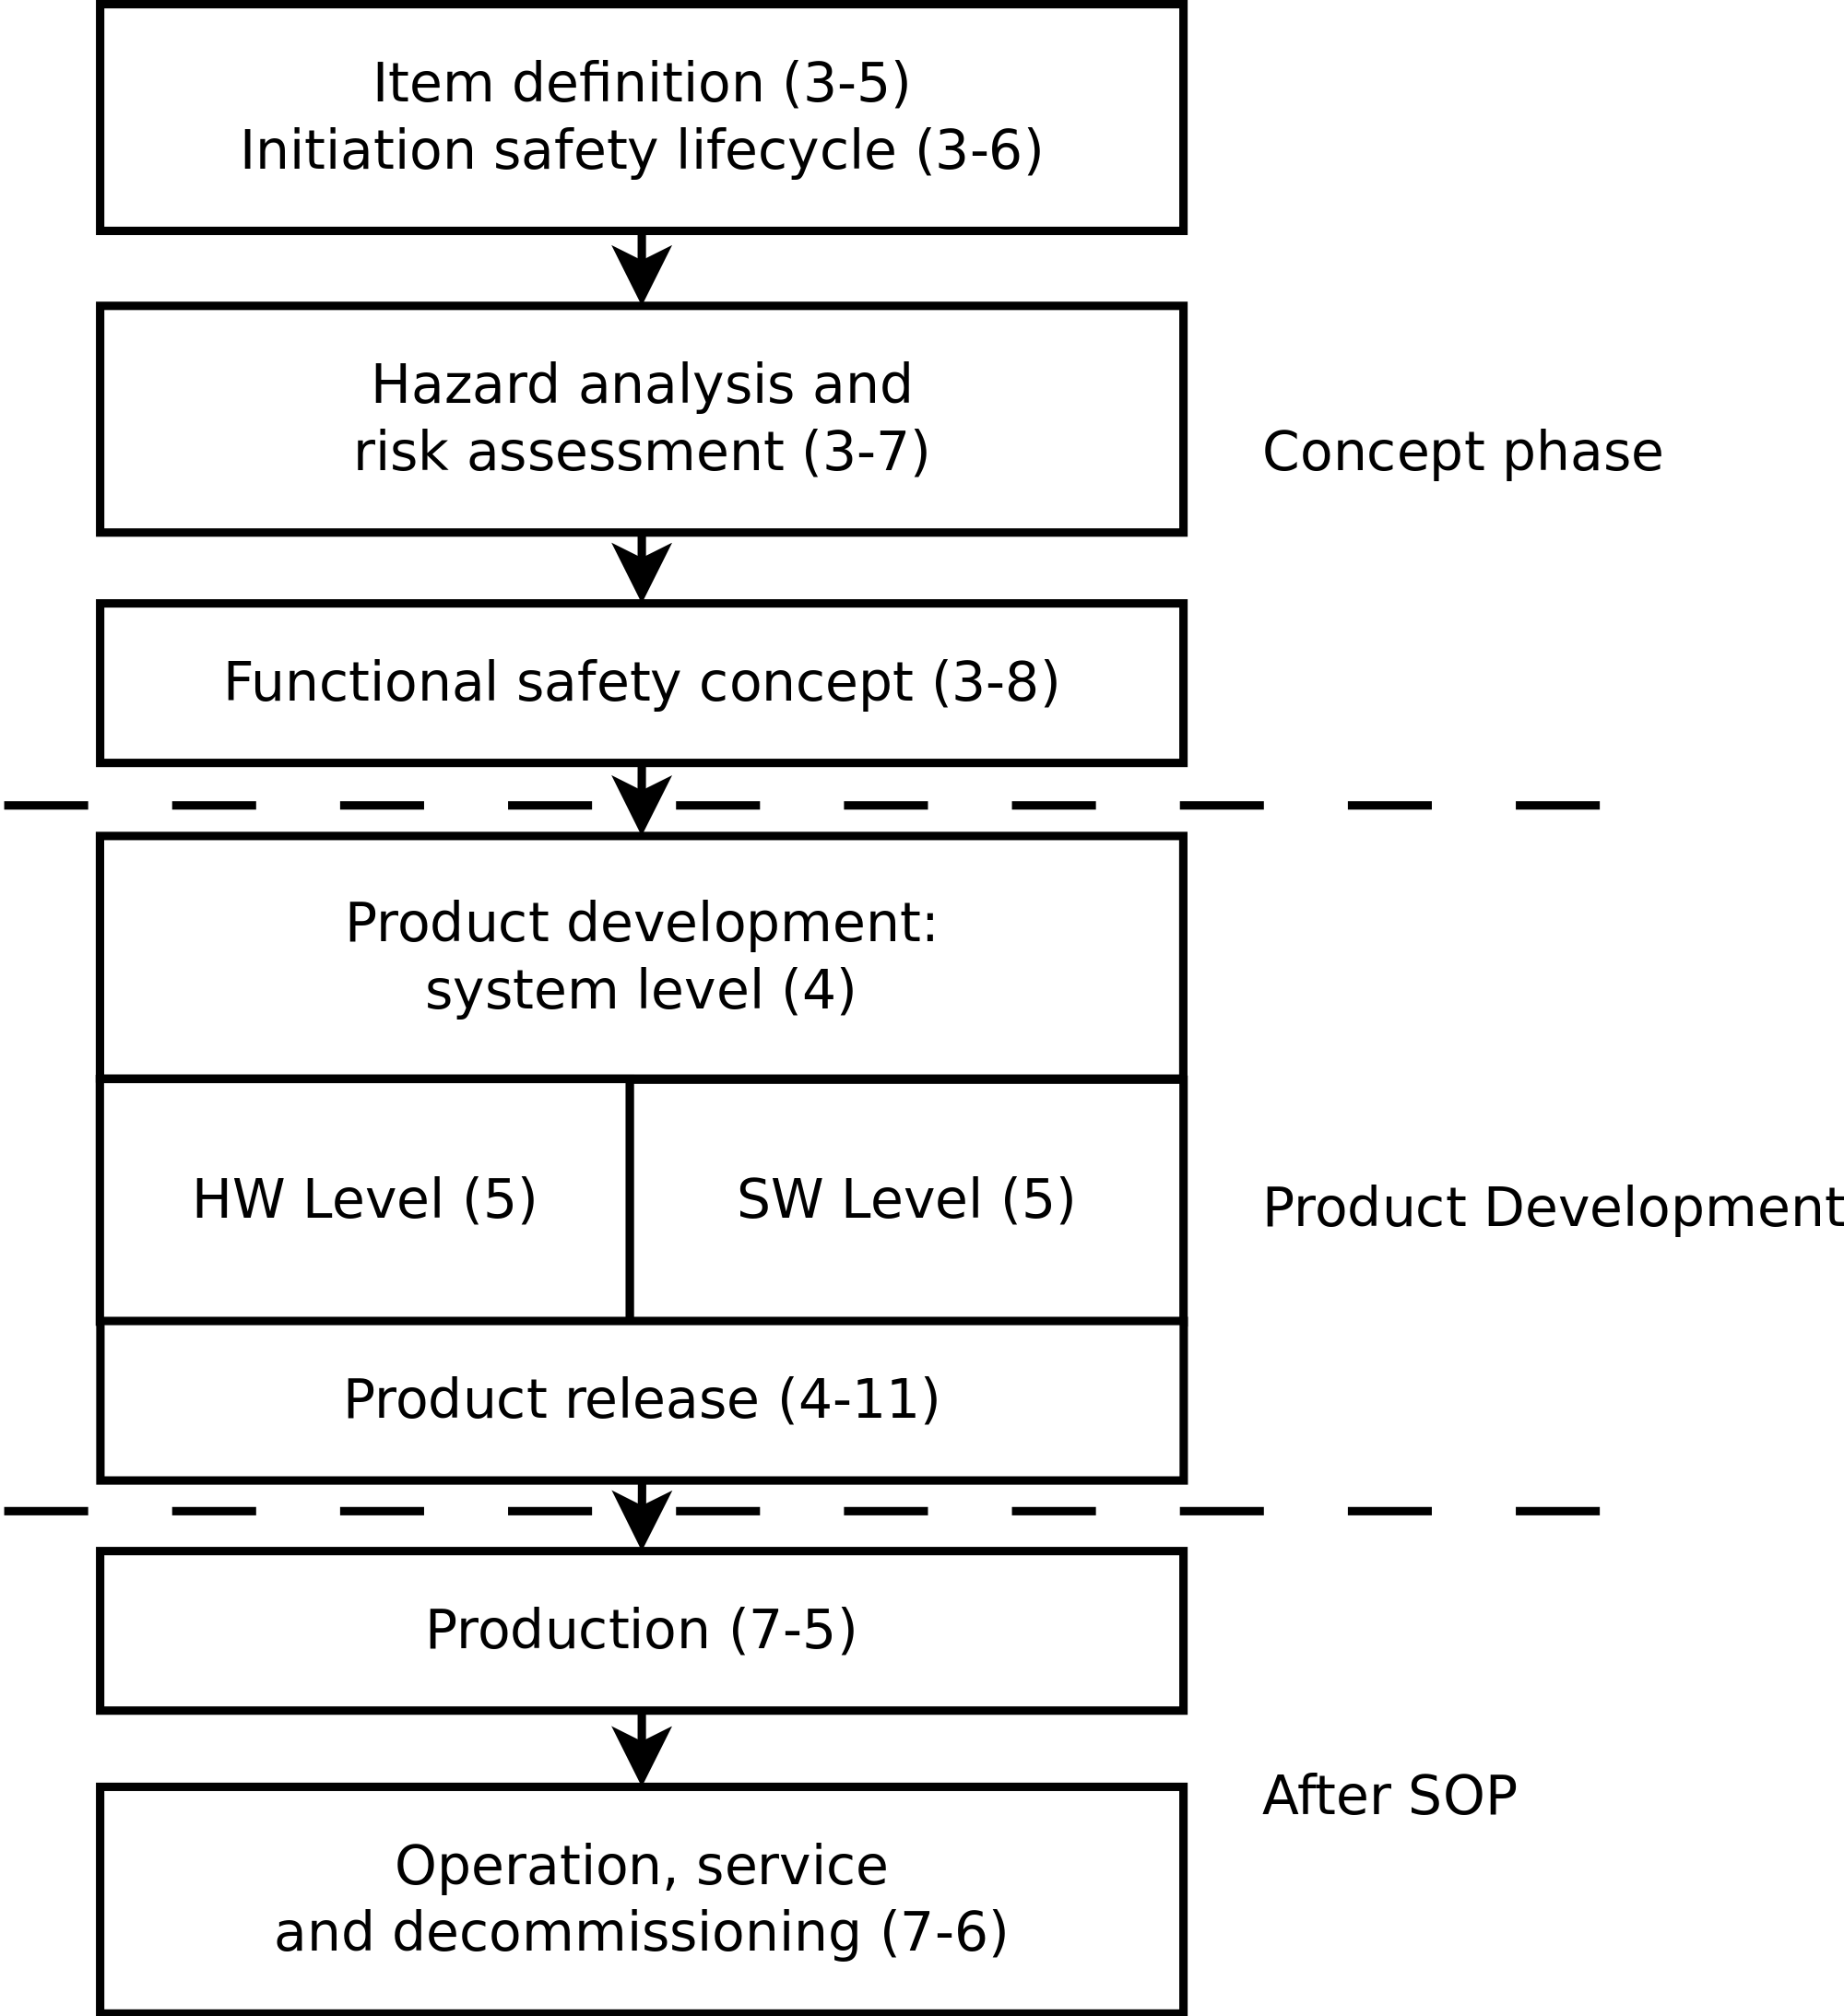
\includegraphics[width=0.75\textwidth]{ISO_26262_Lifecycle}
\caption{Sicheitslebenszyklus nach ISO 26262\cite{iso26262}}
\label{fig:lifecycle}
\end{figure}

Der Lebenszyklus lässt sich in drei Phasen aufteilen. In der \emph{Concept-Phase} werden die Produkt-Anforderungen definiert. Zusätzlich wird hier eine Gefährdungsanalyse und Risikoeinschätzung vorgenommen und ein Sicherheitsplan zur Funktionalen Sicherheit entworfen der alle weiteren Phasen abdeckt.

In der Zweiten Phase, \emph{Product Development}, wird das eigentliche Produkt entworfen. Der Entwurf ist hier in die groben Abschnitte Systementwurf, Hardwareentwurf und Softwareentwurf gegliedert. Am Schluss der Entwicklungsphase steht die Produkt Veröffentlichung. Für alle Abschnitte sind den jeweiligen Kapitel der Norm genauere Informationen zu finden.

Die letzte Phase, \emph{After SOP}\footnote{SOP steht für Start of Production}, betrachtet die Produktion und Auslieferung der Produkte. Der zu Beginn entworfene Sicherheitsplan muss während aller Phasen verbessert und erweitert werden. Dabei muss zu jedem Zeitpunkt Nachvollziehbarkeit und Nicht-Abstreitbarkeit gewährleistet sein. Das bedeutet das jederzeit bekannt ist wer, wann, warum, welche Änderungen vorgenommen hat. Während aller Phasen des Projektes können Reviews, Audits und Sicherheitsassessments durchgeführt werden.

Der genaue Umfang des Managements der Funktionalen Sicherheit wird im Standard nicht festgelegt. Dieser hängt von der Art und Größe des Projektes ab und muss zu Beginn in der Konzept-Phase definiert werden. Einige geforderte Dokumente könnten zum Beispiel sein:

\begin{itemize}
    \item Ausbildungs- und Qualifizierungsnachweise
    \item Sicherheitsplan
    \item Projektplan/Projekthandbuch inklusive der Planung der sicherheitsbezogenen Vorgänge
    \item Review-, Audit- und Assessmentplan
    \item Sicherheitsnachweise
\end{itemize}

\subsection{Gefährdungsanalyse und Risikoeinschätzung}
\label{sec:ISO26262_GundR}
Einer der Kernpunkte der ISO 26262 ist die Gefährdungsanalyse und Risikoeinschätzung. Hierzu werden Vorgehensweisen beschrieben mit Hilfe derer verschiedene Fahrsituationen auf mögliche Fehler untersucht werden können und demeptsprechend Sicherheitseinstufungen vorgenommen werden können. Hierzu wird folgender Ablauf vorgeschrieben:

\begin{itemize}
    \item Ermitteln aller relevanten Fahrzeugzustände und Fahrsituationen
    \item Ermitteln möglicher funktionaler Fehler
    \item Bewerten der Risiken jeder Gefährdungssituation in allen Fahrsituationen
    \item Festlegen der notwendigen Risikominderung (ASIL)
    \item Ableiten der Sicherheitsziele
\end{itemize}

Um nun eine Gefährdungsanalyse durchzuführen wird zu Beginn ein Katalog von Fahrsituationen und möglichen Fehlern erstellt. Anschließend werden alle Fehler aufgrund folgender Eigenschaften bewertet.

\begin{itemize}
    \item Häufigkeit der Fahrsituation (Exposure E; E0 bis E4)
    \item Schwere eines möglichen Schadens (Severity S; S0 bis S3)
    \item Beherrschabrkeit durch den Fahrer (Controllability C; C0 bis C3)
\end{itemize}

Aus diesen drei Eigenschaften wird nun über eine im Standard definierte Tabelle ein \emph{automotive safety integrity level} (ASIL) abgeleitet. Dieser kann die Werte QM, A, B, C und D annehmen. Hierbei steht A für die niedrigsten Anforderungen und D für die höchsten. Die Klasse QM gibt an, dass keine Maßnahmen zur Risikominderung nötig sind.

Im letzten Schritt werden aus dem ASIL Sicherheitsziele abgeleitet. Diese sind den Gefährdungen und Konsequenzen entsprechend zu wählen und im Sicherheitsplan zu beschreiben.


\subsection{Produkt-Entwicklung}
\label{sec:ISO26262_produkt_entwicklung}
Auf genau Prozesse bei der Produkt Entwicklung soll an dieser Stelle nicht eingegangen werden. Allgemein ist jedoch zu sagen, dass die ISO 26262 einige Vorgaben und Empfehlung macht die bei steigendem ASIL an Umfang zunehmen. So können im Bereich der Softwareentwicklung bei ASIL A oder B Anweisungsüberdeckende Tests ausreichend sein, während bei ASIL D umfangreiche Tests nach dem MC/DC\footnote{Modified Condition/Decision Coverage} Prinzip gefordert sind. Im Hardware-Bereich werden außerdem Anforderungen an die Ausfallrate der Systeme gegeben. Um diese zu bestimmen definiert der Standard eine Reihe von Metriken anhand derer die Berechnung der Ausfallraten erfolgt.

Ein wichtiger Punkt der Norm kann außerdem unter dem Leit-Satz: "`bewährte Architekturen wiederverwenden"' zusammengefasst werden. Diese etwas vage Angabe kann verschieden interpretiert werden. Es kann jedoch Allgemein gesagt werden, das alle Standartisierten Techniken als bewährte Architekturen zu sehen sind. Dazu könnten zum Beispiel die ARM-Architektur, die CAN-Schnittstelle oder der POSIX-Standard gezählt werden. Auch Betriebssysteme und Systemarchitekturen wie OSEK/VDX und AUTOSAR gehören hierzu.

Neben den Anforderungen an den Entwicklungsprozess und das Endprodukt werden auch Bedingungen an die verwendeten Software-Werkzeuge gestellt. Diese und einige anderen Anforderungen und Empfehlungen sind unter dem Begriff "`Unterstützende Prozesse"' zusammengefasst. Die Qualifizierung von Software-Werkzeugen relevant, da Fehler nicht nur durch Selbstverschulden sondern auch durch Abhängigkeiten zu Dritt-Software entstehen können. Hierzu unterscheidet die Norm Software-Werkzeuge nach zwei Eigenschaften:

\begin{itemize}
    \item \emph{Tool Impact} (TI0, TI1): Die Wahrscheinlichkeit, durch eine Fehlfunktion des Werkzeugs eine Sicherheitsanforderung zu verletzen.
    \item \emph{Tool Error Detection} (TD1 bis TD4): Die Wahrscheinlichkeit, eine Fehlfunktion des Werkzeugs zu verhindern oder zu erkennen.
\end{itemize}

Diese Eigenschaften bestimmen mittels einer Tabelle einen \emph{Werkzeugvertrauenslevel} (TCL, Tool Confidence Level). Dieser wird eingestuft von TCL1, Werkzeuge die Sicherheitsanforderungen wahrscheinlich nicht verletzen können, bis TCL4 als höchster Vertrauenslevel. So wird eine Textverarbeitungs-Software als TCL1 eingestuft, da diese selbst in schlimmsten Fällen nicht direkt Sicherheit des Endproduktes beeinflusst. Auf der anderen Seite sollte eine Code-Generierungs-Software vermutlich als TCL4 eingestuft werden, da eventuelle Fehler im resultierenden Code verherende Auswirkungen auf die Sicherheit haben können. Zudem können erzeugte Fehler hier nur durch umfangreiche Tests und Code-Reviews erkannt werden.




\subsection{AUTOSAR und ISO 26262}
\label{sec:ISO26262_autosar}
% - Timing Protection, Memory Protection, Program Flow Monitoring
% - Autosar Distributionen die ISO 26262 konform sind bzw. Konformitätsmodule bieten
%   - MICROSAR (Vector Informatics)
% - http://www.elektroniknet.de/automotive/technik-know-how/sicherheitselektronik/article/31185/2/Entwicklung_von_Steuergeraete-Basis-Software_nach_ISODIS_26262/
% - http://www.elektronikpraxis.vogel.de/embedded-computing/articles/342436/
% - Rückwirkungsfreiheit oder „Freedom from Interference“.

Obwohl AUTOSAR und die ISO 26262 auf den ersten Blick keinerlei direkte Verbindungen haben, zeigt sich im weiteren, dass beide Themen zusammen in den letzten Jahren und in der Zukunft stark an Relevanz gewinnen. Dies ergibt sich aus folgendem Auschnitt des Produkthaftungsgesetzes.

% TODO: eines von diesen Zitaten auswählen...
%\begin{quote}
%Erforderlich sind die Sicherungsmaßnahmen, die nach dem im Zeitpunkt des Inverkehrbringens des Produkts vorhandenen neuesten Stand der Wissenschaft und Technik konstruktiv möglich sind [\dots] und als geeignet und genügend erscheinen, um Schäden zu verhindern [\dots].\cite{BGH_Urteil}
%\end{quote}

\begin{quote}
Die Ersatzpflicht des Herstellers ist ausgeschlossen, wenn [\dots] der Fehler nach dem Stand der Wissenschaft und Technik in dem Zeitpunkt, in dem der Hersteller das Produkt in den Verkehr brachte, nicht erkannt werden konnte.\cite{ProdG}
\end{quote}

Da es sich bei AUTOSAR und der ISO 26262 um den aktuellen Stand der Technik handelt, müssen diese Techniken eingesetzt werden, um Regress-Ansprüche vermeinden zu können und das Produkthaftungsgesetz zu befolgen. Dabei kann dies als Umstieg von OSEK/VDX und DIN 61508, gesehen werden. Beide Umstiege gleichzeitig durchzuführen ist ein umfangreicher Schritt, der viel Einsatz erfordert. 

Da es sich bei AUTOSAR um eine Komponenten- und Modul-orientierte Architektur handelt, lässt sich die ISO Norm gezielt auf einzelne Komponenten anwenden wie es auch im Sicherheits-Standard definiert ist. So können einzelne BSW-Module auf deren Risiko-Potenzial geprüft werden und diese anschließend einer Sicherheitsklasse zugeordnet werden. Daraufhin können die entsprechenden Sicherheitsvorkehrungen getroffen werden. Da dies jedoch sehr umfangreich sein kann ist es nicht praktikabel alle Module nach ISO 26262 zu zertifizieren. Vor allem da BSW-Module einfach getauscht und geupdatet werden können, wäre eine jedes mal eine neue Zertifizierung nötig. Diese Schwierigkeit wird von einigen Herstellern umgangen indem nur Teile der Basissoftware zertifiziert wird um damit die Kernpunkte der ISO 26262 abzudecken.

% TODO: Quellen:
% http://www.opensynergy.com/sites/default/files/media/sonstige/COQOS-Datasheet_En.pdf
% http://ww.automotive.elektrobit.com/home/ecu-software/autosar/eb-tresos-product-line/eb-tresos-autocore.html
% http://www.vector.com/vi_microsar_safe_26262_de.html
Sowohl COQOS als auch EB tresos bieten ein ISO 26262 zertifiziertes OS-Modul an. Das Elektorbit OS-Modul ist dabei bis ASIL-D zertifiziert. Hierbei handelt es sich um Mikrokernel mit einer minimalen Funktionalität. Elektrobit bietet zusätzlich ein QM-OS-Modul an, das nicht nach ISO 26262 zertifiziert ist und somit nicht für sicherheitskritische Anwendungen geeignet ist. Eine Absicherung des OS-Moduls kann vor allem die Rückwirkungsfreiheit des Systems garantieren. Ob jedoch auch andere Punkte der ISO abgedeckt sind ist nicht klar. So findet ein Kernpunkt der Norm, die Kommunikation, vor allem in anderen Modulen (Com, PduR\dots) statt. Somit ist eine allgemeine Ende-zu-Ende-Absicherung der Kommunikation nicht möglich.

Das von Vector Informatik eingesetzte Verfahren zur Einhaltung der ISO 26262 beinhaltet drei Module. Das Modul "`SafeExecution"' wird verwendet um Rückwirkungsfreiheit via Laufzeitüberwachung, Speicherschutz und Ablaufkontrolle zu gewährleisten. Dieses ähnelt dem Funktionsumfang der beiden bereits vorgestellten Modelle. Durch das Modul "`SafeCom"' wird zusätzlich eine Ende-zu-Ende-Absicherung der Inntra- und Inter-ECU-Kommunikation vorgenommen. Das dritte Modul, "`SafeSelfTest"', wird verwendet um eine Zyklische Überprüfung der Hardware zu ermöglichen.









%%%%%%%%%%%%%%%%%%%%%%%%%%%%%%% Umsetzung Fallbeispiel %%%%%%%%%%%%%%%%%%%%%%%%%%%%%%%%%%
% Gesamtes Modell darstellen
\chapter{Umsetzung des Fallbeispiels}
\label{sec:Umsetzung_Fallbeispiel}
% TODO







%%%%%%%%%%%%%%%%%%%%%%%%%%%%%%% Virtualisierung %%%%%%%%%%%%%%%%%%%%%%%%%%%%%%%%%%
\section{Virtualisierung}
\label{sec:Virtualisierung_Umgesetzt}
% TODO





%%%%%%%%%%%%%%%%%%%%%%%%%%%%%%% Kommunikation %%%%%%%%%%%%%%%%%%%%%%%%%%%%%%%%%%
\section{Kommunikation Linux und AUTOSAR}
\label{sec:Kommunikation_L_A}
Eine Kommunikation zwischen Linux und AUTOSAR kann auf verschiedene Wege erfolgen. Aus der klassischen Interprozess-Kommunikation sind Techniken wie Dateien, Messages, Semaphoren und Shared Mem bekannt. Diese stehen jedoch unter AUTOSAR nicht zur Verfügung. Stattdessen können Client/Server und Sender/Receiver Interfaces verwendet werden die über verschiedene Schnittstellen nach außen geführt werden können. Im folgenden werden die drei Techniken CAN, Ethernet und VCAN betrachtet. Andere Bus-Systeme wie zum Beispiel LIN oder Flexray sind auch denkbar werden jedach im weiteren nicht näher untersucht. Der hier erwähnte VCAN bezeichnet den virtuellen CAN-Bus der bei Elektrobit tresos eingesetzt wird. Dieser tunnelt die CAN-Botschaften über eine Ethernet Verbindung und kann so CAN-Zugriff auf System ermöglichen die keine CAN-Schnittstelle besitzen. Vor- und Nachteile der Techniken sind im folgenden aufgeführt.

% TODO: hieraus eine Tabelle machen oder vielleicht als texte schreiben?!
\begin{itemize}
    \item CAN
    \begin{itemize}
        \item[$+$] Standard
        \item[$+$] Deterministisch durch Arbitrierung und Zyklische Sender
        \item[$-$] Linux benötigt vollen CAN Zugriff
        \item[$-$] Jedes Linux System CAN-Hardware (Kosten)
    \end{itemize}
    \item Ethernet
    \begin{itemize}
        \item[$+$] Standard
        \item[$+$] Hohe Übertragungsrate
        \item[$+$] AUTOSAR soll "of the shelf"-TCP/IP-Stack verwenden der auch zu Linux kompatibel sein kann\cite[S. 21]{autosar_eth}
        \item[$-$] Kollisionen/Latenz und damit nur bedingt Echtzeitfähig
        \item[$-$] Benötigt AUTOSAR 4.0
    \end{itemize}
    \item VCAN
    \begin{itemize}
        \item[$+$] Baut auf Ethernet auf
        \item[$+$] Gut umsetzbar im Evaluations-Prozess
        \item[$+$] Eigene "Logik" lässt sich im Gateway implementieren (Firewall, Kommunikations Matrix)
        \item[$-$] Nicht geeignet für Prouktiv-Systeme
        \item[$-$] Auf Elektrobit tresos beschränt
        \item[$-$] EB Gateway Protokoll muss implementiert werden
    \end{itemize}
\end{itemize}

% Warum VCAN?!
Sowohl die Kommunikation via Ethernet als auch CAN sind in diesem Projekt nicht weiter relevant, da beide nicht in der verwendeten Version 3.1 von WinCore zur Verfügung stehen. Somit wird in dieser Arbeit der VCAN betrachtet. Dieser ist einfach und flexibel und damit vor allem in den ersten Phasen eines Projektes von Vorteil.

% Deswegen VCAN-API geschrieben
Im Rahmen dieser Master-Arbeit wurde ein VCAN-Gatway in Python entworfen, das sowohl das Senden als auch Empfangen von CAN-Botschaften ermöglicht. Zusätzlich wurde die Funktionalität des von Elektrobit bereitgestellten Closed-Source VCAN-Gateways Reverse-Engineered und leicht erweitert. Im folgenden Kapitel wird die API näher beschrieben.

% Der Quellcode steht unter der LGPL\footnote{Lizenz-Bedingung zu finden unter: \url{http://www.gnu.org/licenses/lgpl-3.0.txt}} und ist im Internet\footnote{VCAN-API Git Repository: \url{https://github.com/erebos42/VCAN_API}} zu finden.


%%%%%%%%%%%%%%%%%%%%%%%%%%%%%%% VCAN-API %%%%%%%%%%%%%%%%%%%%%%%%%%%%%%%%%%
\section{VCAN-Gateway}
\label{sec:VCAN_Gateway}
% Beschreibung der VCAN API
Da das VCAN-Gateway von Elektrobit Closed-Source ist, und damit Änderungen und Erweiterungen nur von Elektrobit vorgenommen werden können, wurde im Rahmen dieser Arbeit eine Alternative entworfen. Als Programmiersprache wurde hier Pyhton gewählt, da bereits Erfahrung hiermit vorhanden ist und eine schnelle Entwicklung möglich ist. Außerdem ist hier zu erkennen das eine Kompplung zwischen zwei Bereichen entsteht. Zum einen die Embedded Welt inklusive CAN-Bus in der fast ausschließlich Assembler, C und C++ vorherschen, und auf der anderen Seite eine Hoch- und Skriptsprache die vor allem einfach und umfangreich ist.

Das VCAN-Gateway besteht aus zwei Teilen. Zum einen die VCAN-API, das Backend, und dem Frontend, bestehend aus dem eigentlichen Gateway und dem VCAN-Viewer.




%%%%%%%%%%%%%%%%%%%%%%%%%%%%%%% Aufbau der ECU %%%%%%%%%%%%%%%%%%%%%%%%%%%%%%%%%%
\section{Aufbau des Bordnetzsteuergerätes}
\label{sec:Aufbau_der_ECU}
Bereits 2011 wurde im Rahmen einer Bachelorarbeit ein Versuchsaufbau zur Ansteuerung von Front-Scheinwerfern erstellt. Dieser Aufbau Bestand aus einem älteren Bordnetzsteuergerät der PQ35 Reihe. Dieses verwendet einen Low-Speed-CAN Bus und ein altes Netzwerk-Management. Dieses NM wird von EB tresos jedoch nicht unterstützt. Aus diesem Grund wurde im Rahmen dieses Projektes ein neues Bordnetzsteuergerät, im weiteren BCM37 genannt, aufgebaut und getestet. Dieses wurde freundlicherweise von VW bereitgestellt. Im Anhang dieser Arbeit (siehe \ref{sec:ecu}) befindet sich eine Dokumentation des Aufbaus und des Bordnetzsteuergerätes.






%%%%%%%%%%%%%%%%%%%%%%%%%%%%%%% Kommunikation %%%%%%%%%%%%%%%%%%%%%%%%%%%%%%%%%%
\section{Kommunikation AUTOSAR und Scheinwerfer}
\label{sec:Kommunikation_A_S}
% TODO
% headlight_final projekt




%%%%%%%%%%%%%%%%%%%%%%%%%%%%%%% NM bei AUTOSAR %%%%%%%%%%%%%%%%%%%%%%%%%%%%%%%%%%
% Netzwerk Management (!)
\section{Einsatz des Netzwerkmanagement}
\label{sec:AutosarNM}
% TODO








%%%%%%%%%%%%%%%%%%%%%%%%%%%%%%% Analyse des Fallbeispiels %%%%%%%%%%%%%%%%%%%%%%%%%%%%%%%%%%
\chapter{Analyse des Fallbeispiels}
\label{sec:Beispiel_Analyse}
% TODO




%%%%%%%%%%%%%%%%%%%%%%%%%%%%%%% Relevanz für die reale Projekte %%%%%%%%%%%%%%%%%%%%%%%%%%%%%%%%%%
% Wie könnte das erarbeitete sinnvoll in der Wirtschaft umgesetzt werden?!
\section{Relevanz für reale Projekte}
\label{sec:Relevanz}
% TODO
% Es gibt bereits einige Embedded Hypervisor
% Multi-Core CPUs und leistungsfähige SOCs sind billig
% Sicherheit (ISO 26262) erfordert viel Aufmerksamkeit
% Kurze "time-to-market" durch Evaluation auf Windows/Linux Platformen
% 



%%%%%%%%%%%%%%%%%%%%%%%%%%%%%%% Benchmark und Betrachtung der Echtzeitfähigkeit %%%%%%%%%%%%%%%%%%%%%%%%%%%%%%%%%%
% 
\section{Benchmark und Betrachtung der Echtzeitfähigkeit}
\label{sec:Benchmark}
% TODO
%
% Teile sollten vielleicht in separate Kapitel?!
%
% - Echtzeitfähigkeit
%   - WinCore
%       - Jitter messen
%       - Kann Windows Echtzeitfähig sein? Auch mit WinCore?
%       - Wie verhält sich der Testaufbau unter Last? CPU-Last auf Windows/WinCore/Linux?
%   - Ethernet
%       - Verhalten unter Last?
%   - Embedded Virt
% - Overhead
%   - WinCore
% - Robustheit
%   - Fehlerhaftes Steuergerät das z.B. dauernd sendet?!
%   - Ethernet






%%%%%%%%%%%%%%%%%%%%%%%%%%%%%%% Sicherheit bei Embedded Virtualisierung %%%%%%%%%%%%%%%%%%%%%%%%%%%%%%%%%%
\section{Sicherheitsbetrachtung des Fallbeispiels}
\label{sec:Sicherheit_Beispiel}
% TODO
% krypto instanz in embedded hyp











%%%%%%%%%%%%%%%%%%%%%%%%%%%%%%% Zusammenfassung %%%%%%%%%%%%%%%%%%%%%%%%%%%%%%%%%%
\chapter{Fazit und Ausblick}
\label{sec:FazitAusblick}
% TODO










%%%%%%%%%%%%%%%%%%%%%%%%%%%%%%%%%%% Anhang %%%%%%%%%%%%%%%%%%%%%%%%%%%%%%%%%

\appendix
\part*{Anhang}

% This file contains sensitive information that is not shared on GitHub!!!
% If you don't have the appendix.tex, then this line has to be deleted.





%%%%%%%%%%%%%%%% VCAN-API %%%%%%%%%%%%%%%%%%%%
\chapter{VCAN-API}
\label{sec:vcan_api}
Dieses Kapitel beschreibt die im Laufe des Projektes erstellte Software zur Kommunikation per virtuellem CAN. Alle Informationen über das Protokoll wurden per Reverse Engineering ermittelt.
% TODO:


\section{Protokoll}
\label{sec:vcan_protokoll}
% TODO:
% Protokoll, duh?!



\section{Projekt Struktur}
\label{sec:vcan_struktur}
% TODO:
% Dateien, Klassen
% Abhängigkeiten
\begin{description}
    \apiitem{./vcan\_api/}
    Dieses Verzeichnis enthält die gesamte VCAN-API.
    \begin{description}
        \apiitem{./vcan\_api/\_\_init\_\_.py}
        VCAN-API Python Pyackage.
        \apiitem{./vcan\_api/PCANBasic.py}
        API zur Nutzung des PEAK-PCAN-USB-Adapters. Diese Datei stammt von PEAK.
        \apiitem{./vcan\_api/vcan\_client.py}
        Enthält die Klasse VCANClient.
        \apiitem{./vcan\_api/vcan\_config.py}
        Enthält die Klasse VCANConfig.
        \apiitem{./vcan\_api/vcan\_config.xsd}
        XML-Schema für Firewall-Konfigurationen.
        \apiitem{./vcan\_api/vcan\_exception.py}
        Enthält die Klasse VCANException.
        \apiitem{./vcan\_api/vcan\_gateway.py}
        Enthält die Klasse VCANGateway.
        \apiitem{./vcan\_api/vcan\_message.py}
        Enthält die Klasse VCANMessage und einige Konstanten um diese zu Nutzen.
    \end{description}
    \apiitem{./gateway.py}
    Ein simples Gateway mit grafischer Oberfläche.
    \apiitem{./gateway\_rules.xml}
    Eine Beispiel-Konfiguration der im Gateway eingebauten Firewall-Regeln.
    \apiitem{./sample\_*.py}
    Verschiedene Python-Beispiele, die die VCAN-API nutzen.
\end{description}


\section{Gateway API}
\label{sec:vcan_gateway_api}

% class VCANGateway
\begin{description}
    \apiitem{class VCANGateway(receive\_callback=None, connection\_callback=None)}
    Das Gateway nimmt Verbindungen von Clients entgegen und verteilt eingehende Botschaften an alle angemeldeten Clients weiter.
    \begin{description}
        \apiitem{start\_gateway(host='127.0.0.1', port=10020, rulesfile='')}
        Startet das Gateway auf IP \texttt{host} und dem Port \texttt{port}. Auf dem ausführenden Rechner muss ein Netzwerk-Interface mit der entsprechenden IP existieren. Der Port darf nicht durch eine andere Anwendung belegt sein. Optional kann eine Regeldatei angegeben werden um Firewall-Regeln zu definieren. Dies ist noch experimentell.
        \apiitem{stop\_gateway()}
        Stoppt das Gateway wieder. Anschließend kann mittels der \texttt{start\_gateway} Methode wieder gestartet werden. Es werden jedoch alle Verbindungen getrennt, und die Host IP muss ein weiteres mal angegeben werden.
        \apiitem{connect\_other\_gateway(host, port=10020)}
        Ein Gateway kann sich zu einem anderen Gateway verbinden um ein Netz zu bilden. Das Ziel-Gateway muss unter der IP \texttt{host} und dem Port \texttt{port} erreichbar sein. Diese Methode ist hilfreich, wenn zum Beispiel eine Firewall eingehende Verbindungen verbietet oder ein Gateway unter Linux mit einem Windows-Gateway verbunden wird, um den PCAN nutzen zu können.
        \apiitem{pcan\_init()}
        Initialisiert den ersten gefundenen PEAK-PCAN USB-Dongle mit einer Baud-Rate von 500kbaud. Das gwählte USB-Interface und die Baud-Rate können zur Zeit nur im Code geändert werden. PCAN Support ist im Moment nur unter Windows vorhanden und wird ansonsten durch eine VCANException markiert.
        \apiitem{pcan\_uninit()}
        Deinitialisiert den PEAK-PCAN USB-Dongle.
    \end{description}
\end{description}

% class VCANConfig
\begin{description}
    \apiitem{class VCANConfig(rulesfile)}
    Diese Klasse wird verwendet um Firewall-Regeln im Gateway zu implementieren. Hierzu wird eine XML-Datei mit Regeln übergeben. Diese Datei muss dem beiligenden Schema \texttt{vcan\_config.xsd} entsprechen. Das Gateway ist dafür verantwortlich die entsprechenden Überprüfungen beim Senden und Empfangen durchzuführen.
    \begin{description}
        \apiitem{is\_send\_allowed(ip, can\_id)}
        Überprüft ob die IP \texttt{ip} eine Botschaft mit der ID \texttt{can\_id} senden darf. Gibt True zurück falls erlaubt, und False falls verboten.
        \apiitem{is\_receive\_allowed(ip, can\_id)}
        Überprüft ob die IP \texttt{ip} eine Botschaft mit der ID \texttt{can\_id} empfangen darf. Gibt True zurück falls erlaubt, und False falls verboten.
    \end{description}
\end{description}

% class VCANException
\begin{description}
    \apiitem{class VCANException(value)}
    Exception der VCAN-API. Wird beim Gateway verwendet, falls die PCAN-Verbindung nicht initialisiert werden kann.
\end{description}




\section{Client API}
\label{sec:vcan_client_api}

% class VCANClient
\begin{description}
    \apiitem{class VCANClient(q\_length=1024)}
    Diese Klasse kann verwendet werden, um Zugriff auf den VCAN zu erhalten. Es bietet Funktionen um eine Verbindung aufzubauen und zu schließen. Außerdem können Botschaften empfangen und gesendet werden. Standardmäßig erfolgt das Empfangen auf Polling-Basis. Hierzu wird eine Queue der Länge \texttt{q\_length} angelegt. Der Anwender ist verantwortlich die eingehenden Daten häufig genug zu pollen. Alternativ kann für das Empfangen eine Callback-Funtion angegeben werden.
    \begin{description}
        \apiitem{connect(ip, port=10020, receive\_data=True, callback=None)}
        Verbindet den Client mit einem Gateway auf IP \texttt{ip} und Port \texttt{port}. Über den Schalter \texttt{receive\_data} kann das Empfangen von Botschaften deaktiviert werden. Der Parameter \texttt{callback} kann verwendent werden um eine Funktions-Referenz zu übergeben, die empfangene Botschaften direkt verarbeitet. Wirft \texttt{VCANException} falls keine Verbindung hergestellt werden kann.
        \apiitem{close(sleep\_time=0.5)}
        Schließt die aktuelle Verbindung. Der Parameter \texttt{sleep\_time} wird verwendet um nach dem Schließen der Verbindung einen Moment zu warten. Damit werden Eigenheiten des EB-Gateways und der AUTOSAR-Anwendungen ausgeglichen, da es ansonsten zu Fehlern kommen kann. Die Angabe erfolgt in Sekunden.
        \apiitem{get\_received\_item()}
        Gibt die älteste empfangene Botschaft zurück. Falls die Queue leer ist wird \texttt{None} zurückgegeben. Diese Methode muss im Polling-Betrieb häufig genug aufgerufen werden, um Daten-Verlust zu vermeiden.
        \apiitem{send(message, sleep\_time=0.2)}
        Sende die Botschaft \texttt{message} zum verbundenden Gateway. Die Botschaft kann sowohl als Binär-String, als auch als VCANMessage vorliegen. Der Parameter \texttt{sleep\_time} wird verwendet um Fehler zu vermeiden indem nach dem Senden ein Moment gewartet wird. Falls nur Applikation angebunden sind, die die VCAN-API nutzen kann dieser Wert auf 0 gesetzt werden. AUTOSAR-Applikation haben jedoch Probleme mit zu geringen Warte-Zeiten und können Botschaften verlieren oder sogar abstürzen. Die Angabe erfolgt in Sekunden. Falls der Client zu keinem Gateway verbunden ist, wird eine \texttt{VCANException} geworfer.
    \end{description}
\end{description}

% class VCANMessage
\begin{description}
    \apiitem{class VCANMessage()}
    Repräsentiert eine Botschaft in der VCAN-API. Der Konstruktur generiert eine leere Botschaft. Diese kann entweder über \texttt{set\_parameters()} von Hand mit Parametern gefüllt werden, oder über \texttt{parameters\_from\_string()} von einer eingehenden Nachricht aus einem Binär-String.
    \begin{description}
        \apiitem{set\_parameters(can\_id,  data, system, channel, dlc=None)}
        Setzt die Parameter der Nachricht entsprechend den Parametern. Parameter \texttt{can\_id} gibt die ID der Botschaft an. Die Nutzdaten sind werden in \texttt{data} erwartet und müssen als Liste übergeben werden. Die Parameter \texttt{system} und \texttt{channel} geben das entsprechende System und den Kanal an. Standard-Werte sind CAN und Kanal 0. Weitere Möglichkeiten sind in der Datei \texttt{vcan\_message.py} als Konstanten hinterlegt. Der letzte Parameter, \texttt{dlc}, gibt die Länge der Daten an. Falls \texttt{None} übergeben wird, wird die Länge des Daten-Arrays verwendet.
        \apiitem{parameters\_from\_string(m\_string)}
        Setzt die Parameter der Nachricht anhand des Binär-Strings \texttt{m\_string}. Diese entsprechen direkt dem TCP-Paket und können hierdurch in eine VCAN-API-konforme Form gebracht werden.
        \apiitem{to\_sendable\_string()}
        Wandelt die Botschaft in einen Binär-String um, der per TCP versendet werden kann.
    \end{description}
\end{description}

% class VCANException
\begin{description}
    \apiitem{class VCANException()}
    Exception der VCAN-API. Wird geworfen falls die Verbindung zu einem Gateway scheitert, oder eine Nachricht gesendet wird obwohl keine Verbindung besteht. Außerdem siehe \ref{sec:vcan_gateway_api}
\end{description}




\section{Beispiel Anwendungen}
\label{sec:vcan_beispiele}

















% TODO: BSW-Modul-Liste; Grafische Notation (AUTOSAR, SPEM); 


% Alles hier nach hat keine Nummerierung mehr...
\backmatter



\chapter{Beigelegte CD}
\label{sec:BeigelegteCD}



%%%%%%%%%%%%%%%%%%%%%%% Erklärung und CD %%%%%%%%%%%%%%%%%%%%%%%%%%%%%
\chapter{Erklärung}
\label{sec:Erklärung}
Hiermit erkläre ich, dass ich die vorliegende Arbeit selbstständig und nur unter Verwendung der angegebenen Quellen und Hilfsmittel erstellt habe.
\vspace{2.5cm} \par
Wolfenbüttel, den % TODO


% Alle Einträge zum Glossar hinzufügen und Glossar/Akronymliste printen
\glsaddall
\printglossaries


%%%%%%%%%%%%%%%%%%%%%%%%%%%%%%% Bibliographie %%%%%%%%%%%%%%%%%%%%%%%%%%%%%%
% \setbibpreamble{Die Quellenangaben sind alphabetisch nach den Namen der Autoren sortiert.
% Bei mehreren Autoren wird nach dem ersten Autor sortiert.\par\bigskip\bigskip}
%
% Quellen, die nicht direkt zitiert wurden, aber trotzdem hier erscheinen sollen!
%\nocite{tbinformatik}\nocite{tb_et2000}\nocite{tb_mathe1999}
\nocite{*}
%
\begin{singlespace}
\bibliographystyle{natdin}	% alphadin, plaindin, abbrvdin, unsrtdin, natdin
					            % germbib: gerabbrv, geralpha, gerplain, gerunsrt, gerapali, gerxampl
                           		% plainnat, abbrvnat, unsrtnat
                           		% Am besten geeignet: natdin
                           		% oder was ist mit dinat
                           		% ???apalike???
\bibliography{literature}
\end{singlespace}
%%%%%%%%%%%%%%%%%%%%%%%%%%%%%%%%%%%%%%%%%%%%%%%%%%%%%%%%%%%%%%%%%%%%%%%%%%%%

\end{document}


